\documentclass[../ClassicThesis.tex]{subfiles}
\begin{document}

\newcommand\myNotes[1]{\textcolor{red}{#1}}
\newcommand{\note}[1]{\myNotes{#1}}
\newcommand{\class}[1]{\emph{#1}}
\newcommand{\name}[1]{\textit{#1}}

% put this into the intro
% \platener is a web application,
% converts input {\threedmodels} into {\svgfiles}

% ************************************************
\chapter{Architecture}
\label{ch:architecture}
% ************************************************

In this chapter we outline the architecture and composition of the
application {\platener}. Therefore, we look at concepts of graphics
programming in web-environments in Section~\ref{sec:cg-web}. Then, we
explore the structure of our software from two points of view. At
first, we present {\convertify} in
Section~\ref{sec:framework-convertify}. {\convertify} is the
web-framework in which {\platener} is implemented. Secondly, we
explain the details of {\platener} in
Section~\ref{sec:application-platener}.

% \note{weiss nicht ganz was die zwei naechsten absaetze
%   bringen...}

% With a framework like {\convertify} we can implement generic
% {\threedmodel} manipulation web-applications. {\threedmodel}
% manipulation means restructuring the model geometry in such a way,
% that it can be used for a new purpose - apart from visualization on
% computer screens. Such manipulations include converting the
% {\threedmodel} for physical output devices like {\threedprinter}s or
% {\lasercutter}s. For example, {\brickify} creates models consisting of
% 3D-printed parts and
% {\lego}-assembled\footnote{\url{http://www.lego.com}} parts. Thus,
% applications like
% {\brickify} can be built with {\convertify}.

% {\platener} is an application implemented in the framework {\convertify}.
% Using a framework helps us focusing on the algorithmic challenges of
% converting arbitrary {\threedmodel}s into physical, laser-cut output.
% \note{letzter satz: sagt nichts aus?}

\section{Computer Graphics in Web-Environments}
\label{sec:cg-web}
% ************************************************

In this section we give a brief overview of graphics programming
fundamentals in general and in web-environments. These fundamentals
are the concepts of {\threedmodel} data representation in
Section~\ref{sub:model-representation} and render loops and scene
graphs in Section~\ref{sub:render-and-graph}.

\subsection{{\threedmodel} Representation}
\label{sub:model-representation}

This section explains which data structures and disk-formats are used
to represent {\threedmodel}s. First, we explain the terminology of
meshes. Secondly, we look at the {\stlfile} format.

The model geometry is represented by a set of connected
polygons, approximating the model surface. These connected
polygons form a mesh. Figure~\ref{fig:term-mesh:mesh} shows
a mesh. We use triangles as polygons, because then we
benefit from hardware acceleration. A triangle in the mesh
is called face. Each face is described by a list of three
coordinates in 3D-space. Such a coordinate is called vertex
\cite[p.~3]{cg-intro}. An edge is the line between two
connected vertices. Figure~\ref{fig:term-mesh:face}
illustrates the terminology.

\begin{figure}[h]
  \centering
  \begin{subfigure}[b]{0.49\textwidth}
    \centering
    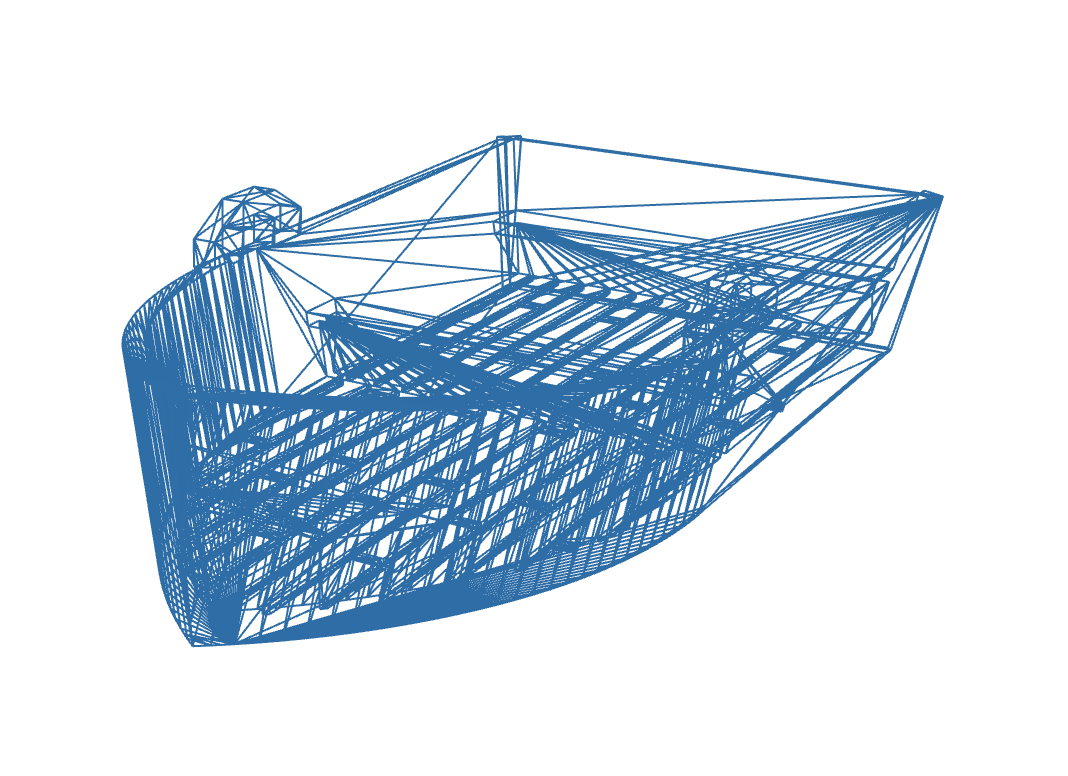
\includegraphics[width=\textwidth]{03-architecture-boat}
    \caption{A triangle mesh of a rowboat.}
    \label{fig:term-mesh:mesh}
  \end{subfigure}
  \begin{subfigure}[b]{0.49\textwidth}
    \centering
    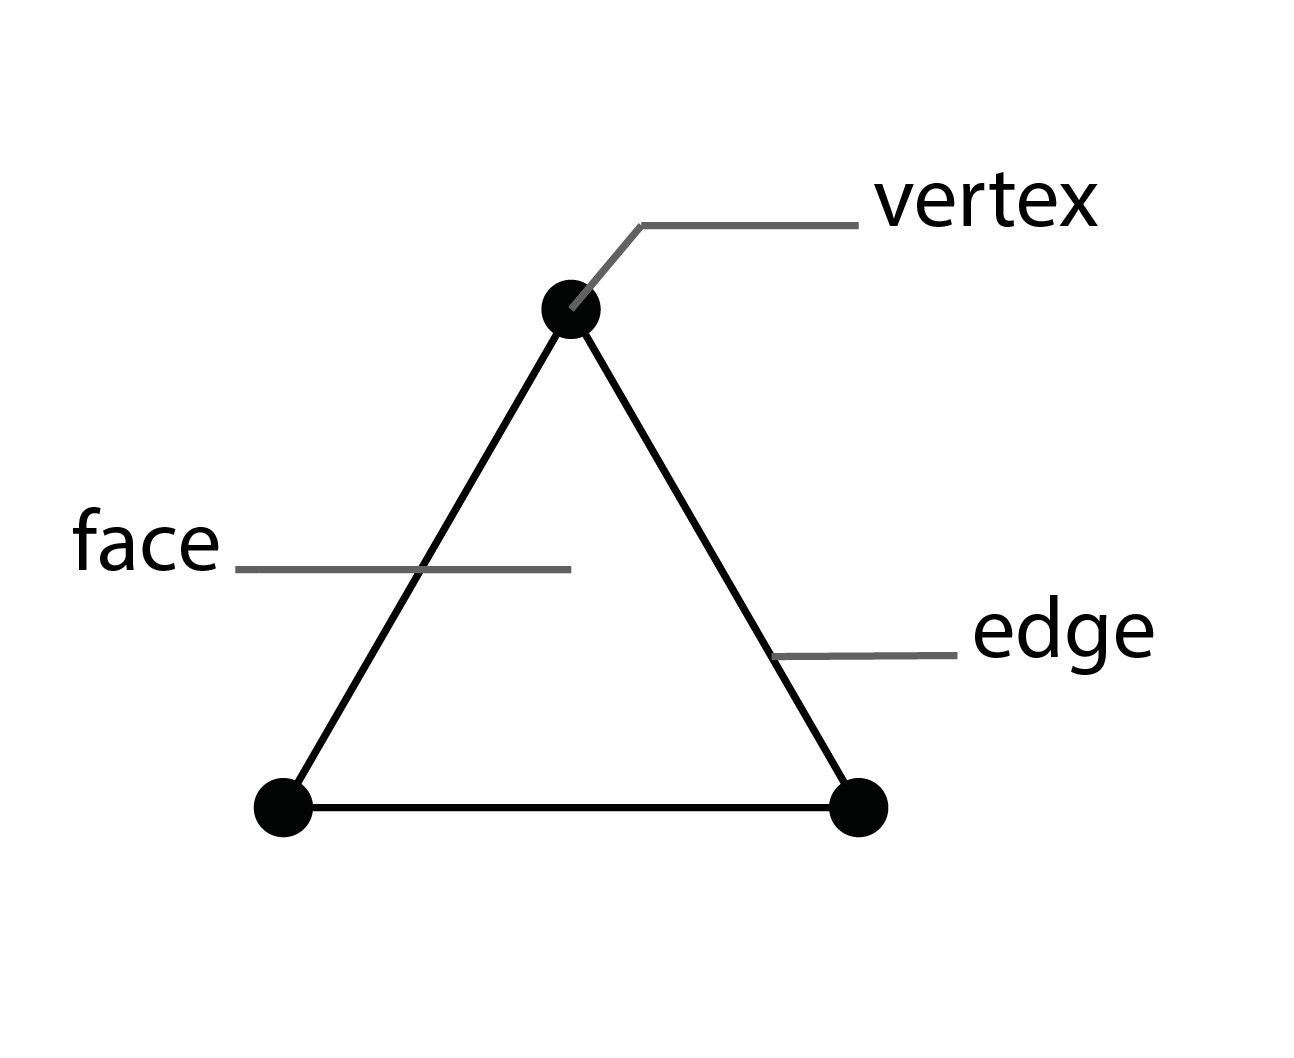
\includegraphics[width=\textwidth]{03-architecture-mesh-terminology}
    \caption{A single face with vertices and edges.}
    \label{fig:term-mesh:face}
  \end{subfigure}
  \caption{Terminology of a Mesh}
  \label{fig:term-mesh}
\end{figure}

We only support geometry which is arranged in two-manifold meshes.
Two-manifoldness is a constraint on the mesh, which requires each egde
to exactly touch two neighboring faces. Figure~\ref{fig:non-manifold}
shows a comparison of a manifold and non-manifold part of a mesh. It
follows then, that each triangular face has to have three adjacent
faces. Thus, the constraint enforces the mesh to be a fully connected
graph without holes \cite[p.~28]{master-thesis}. We require
two-manifoldness to make
sophisticated assumption when designing the conversion algorithms.

\note{make own figure for non-manifold mesh}

\begin{figure}[h]
  \centering
  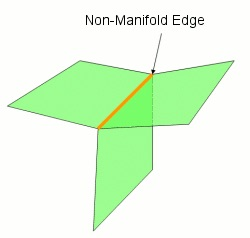
\includegraphics[width=0.6\textwidth]{03-architecture-non-manifold}
  \caption{A non-manifold cutout of a mesh.}
  \label{fig:non-manifold}
\end{figure}

The Standard Tessellation Language (STL) format is a common file
format for {\threedmodel} representation in the context of
{\threedprinting}. We support the {\stlfile} format, because our goal
is to make models, built for a {\threedprinter}, available for the
{\lasercutter}. An {\stlfile} consists of a list of faces associated
with their face normal. The face normal determines the orientation of
the face. We need the face normal, because from the vertices only, we
cannot say in which direction the face points. Each face is a list of
vertices. A vertex is described by three floating point numbers.
Listing~\ref{alg:stl-file} shows an {\stlfile} in ASCII encoding. For
saving disk-space, the file is mostly stored in a binary format
\cite[p.~8]{stl-file}.

\begin{listing}
\centering
\begin{CVerbatim}
solid name
 facet normal n1 n2 n3
  outer loop
   vertex p1x p1y p1z
   vertex p2x p2y p2z
   vertex p3x p3y p3z
  endloop
 endfacet
endsolid name
\end{CVerbatim}
\caption{General format of a STL-file in ASCII encoding.}
\label{alg:stl-file}
\end{listing}

Reconstructing the original {\threedmodel} from an {\stlfile} does not
always result in one-to-one solution. The vertices are stored with
floating point numbers instead of referring to the same vertex with an
index. Thus, we have to assume, that two overlapping points represent
an identical vertex. We use the library {\meshlib} to create an
indexed face-vertex-mesh from the possibly ambiguous {\stlfile}. With
{\meshlib} we can convert the face-vertex-mesh representation to a
{\threejs} geometry. With a {\threejs} geometry, we can render a
{\threedmodel} in {\convertify}.

To support a variety of {\threedprinter} optimized models, we use the
{\stlfile} format. We import the files with the {\meshlib} library.
The imported face-vertex-mesh structure is then converted for usage
with {\threejs}. The section below, explains how the {\threejs}
representation is displayed on the screen.

\subsection{Render Loop and Scene Graphs}
\label{sub:render-and-graph}

To understand how {\convertify} and {\platener} work, we have to
familiarize with the concepts of rendering and scene graphs first.

A typical pattern in graphics software is the render loop.
Rendering is the process of turning the {\threedmodel}
representation into an array of pixels which can be
displayed on the screen~\cite[p.~2]{intro-cg}. We have to
render the {\threedmodel} in a continuous loop, because we
do not want to produce a single static image. The render
loop pattern consists of three steps: processing input,
updating the {\threedmodel} representation and
rendering~\cite{gamedev-gameloop}.
Figure~\ref{fig:render-loop} shows an exemplary flow.

\begin{figure}[h]
  \centering
  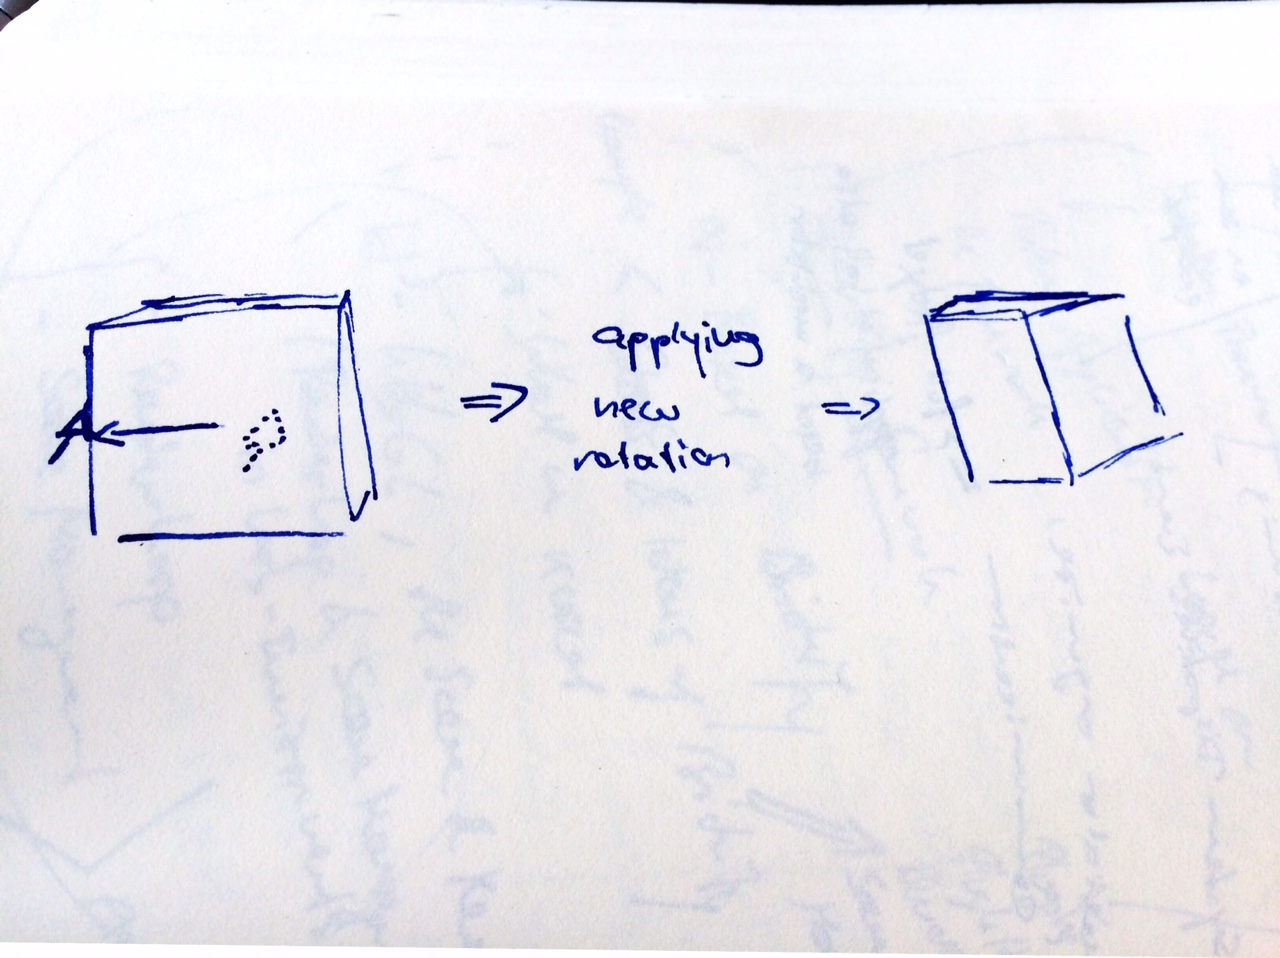
\includegraphics[width=1\columnwidth]{03-architecture-render-loop}
  \caption{Touch input is processed by the render loop.}
  \label{fig:render-loop}
\end{figure}

Each object is part of a scene. A scene is the visual space, in which
the rendered objects can be seen. Instead of rendering each vertex of
the model directly to the scene, we use representations of objects,
which are organized in a hierarchical data structure. We refer to this
hierarchical structure as scene graph\ref{}\myNotes{reference scene
  graph data structure}. A simple scene graph is depicted in
Figure~\ref{}. The shown graph contains a box as single root node. The
sides of the box are children of the root node. With this abstraction
we can easily apply transformations to parts of the model only,
without necessarily touching each face or vertex. Every object, that
is recognized by {\convertify} is part of a scene graph.

\begin{figure}[H]
  \centering
  \begin{subfigure}[b]{0.49\textwidth}
    \centering
    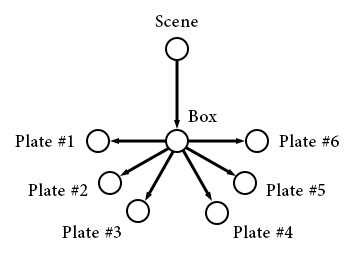
\includegraphics[width=\textwidth]{03-architecture-scene-graph-abstract}
    \caption{Graph notation of the composed box.}
    \label{fig:scene-graph:abstract}
  \end{subfigure}
  \begin{subfigure}[b]{0.49\textwidth}
    \centering
    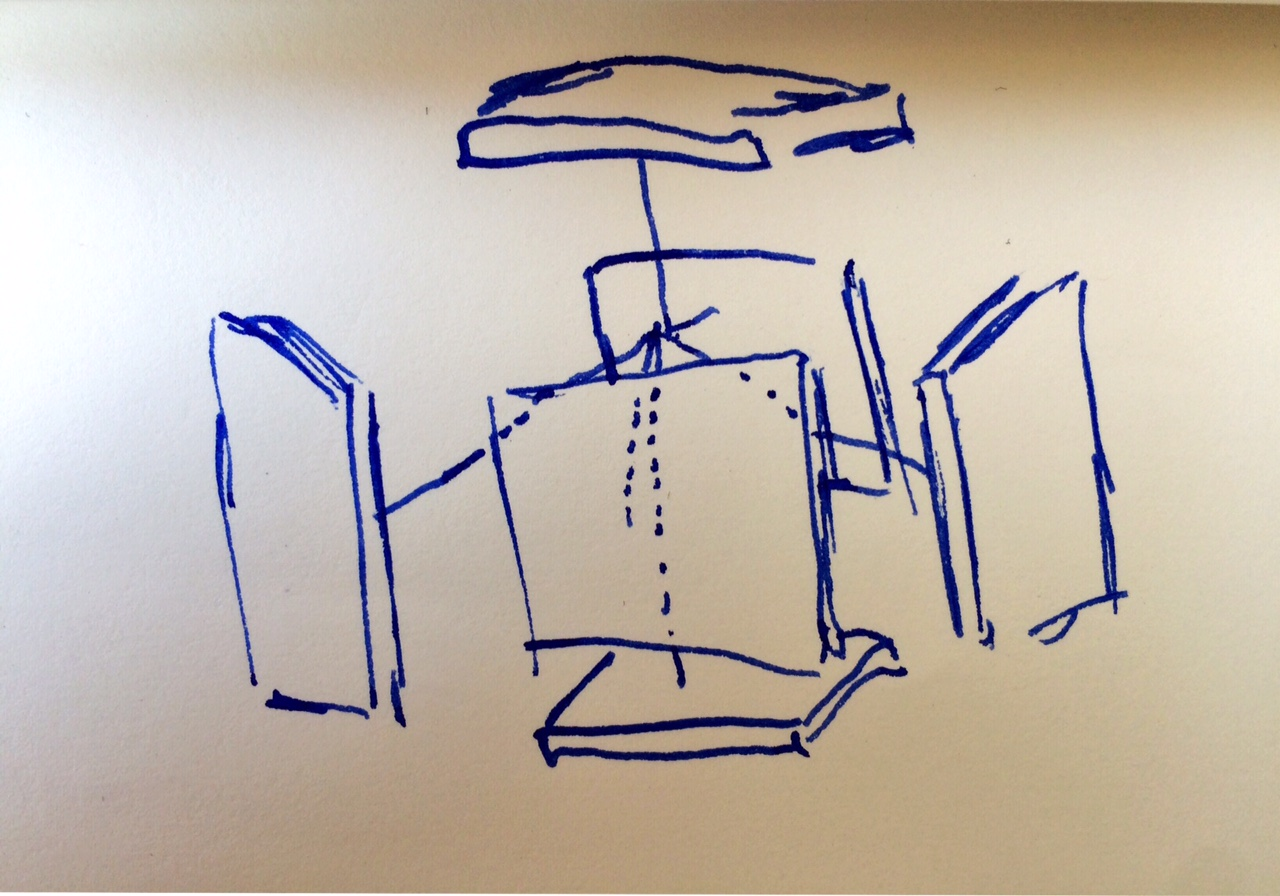
\includegraphics[width=1\textwidth]{03-architecture-scene-graph-visual}
    \caption{Rendered box, showing decomposition into plates.}
    \label{fig:scene-graph:visual}
  \end{subfigure}
  \caption{A scene graph showing a box, composed of plates.}
  \label{fig:scene-graph}
\end{figure}


The framework {\convertify} uses common computer graphics
patterns like render loops and scene graphs. With the help
of WebGL and {\threejs} we are able to bring these concepts
into a web-environment.


\section{Convertify}
\label{sec:framework-convertify}

In this section we present {\convertify}, a web-framework
for working with {\threedmodel}s. We will explain core
features of {\convertify} in
Section~\ref{sec:convertify-core-features.}. Then we will
dive into its plugin system in
Section~\ref{sec:plugin-system}. {\convertify} is based on
previous work by \citeauthor{brickify-thesis}. We will give
a short comparison of their work with {\convertify} in
Section~\ref{sec:brickify-comparison}.


% We explain the work and
% concepts of \citeauthor{brickify-thesis} in
% Section~\ref{sec:based-brickify}. Then we outline, how we
% incorporated the previous work into {\convertify} in
% Section~\ref{sec:reuses-brickify} and
% Section~\ref{sec:plugin-system}.

\subsection{Introduction to the Core System of {\convertify}}
\label{sec:convertify-core-features}

In this section we present the core system of {\convertify}.
{\convertify} helps to build WebGL applications by providing
abstractions to the rendering engine and by composing
features into plugins. We will focus on important design
decisions, which are scene management, rendering and
plugins.

\subsubsection{{\threedmodel}s Are Managed in a Flat Scene
  Graph}

A flat scene graph is a scene graph with only one level of
hierarchy. Thus, our entities in the scene graph do not have
any children. We only need a flat scene graph, because we
only have to manage and access the input models.

We implement the flat scene graph using \class{Nodes}.
\class{Nodes} are abstract objects, which represent an
entity in our scene graph. Each \class{Node} references an
input model and transforms. The input model is a
face-vertex-mesh, that is either used for rendering or used
by algorithms for further computation. Transforms
describe spatial properties like position, scale or
rotation.

All \class{Nodes} are part of a \class{Scene}. A
\class{Scene} holds reference of \class{Nodes}, so we can
access the input models for later usage. \class{Nodes} are
added to or removed from the \class{Scene} via the
\class{SceneManager}. Figure~\ref{fig:scene-graph} shows how
these classes relate.

\begin{figure}[h]
  \centering
  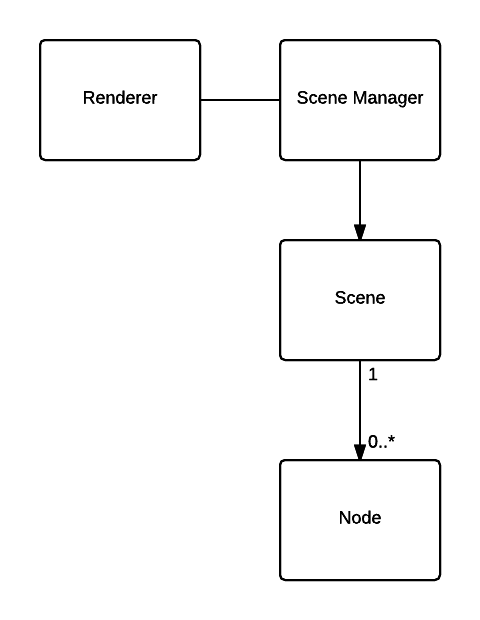
\includegraphics[width=0.6\textwidth]{03-architecture-scene-graph}
  \caption{Relation of scene graph components}
  \label{fig:scene-graph}
\end{figure}

\subsubsection{{\threedobject}s Are Rendered with
  {\threejs}}

% A \class{Scene} contains all \class{Nodes} that reference an
% input model.
Though \class{Nodes} represent entities in the scene of
{\convertify}, only {\threejs} objects can actually be
rendered. Such {\threejs} objects are instances of
\class{THREE.Object3D}\footnote{\url{http://threejs.org/docs/#Reference/Core/Object3D}}.
This is a generic object, which can be rendered into a WebGL
scene. These \class{THREE.Object3D} will be displayed on the
screen. The scene graph of {\threejs} is not flat. A
\class{THREE.Object3D} can have a hierarchy of objects of
any size.

We use a \class{Renderer} to bring {\threejs} entities to
the screen. The \class{Renderer} sets up a WebGL context and
initializes {\threejs}. {\convertify} associates each
\class{Node} with one or more \class{THREE.Object3D}. The
\class{Renderer} traverses the hierarchy of each associated
\class{THREE.Object3D} and renders it. The \class{Node}
transforms are thereby applied to the {\threejs} entities.

Figure~\ref{fig:nodes-and-three} shows the
\class{THREE.Object3D} in the context of \class{Nodes} and
the \class{Renderer}.

\begin{figure}[h]
  \centering
  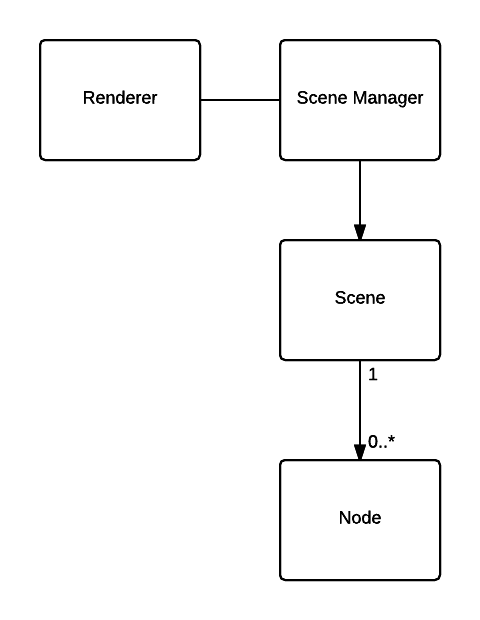
\includegraphics[width=0.6\textwidth]{03-architecture-scene-graph}
  \caption{\class{Nodes} and associated \class{THREE.Object3D}}
  \label{fig:nodes-and-three}
\end{figure}

\subsubsection{Convertify Emits System Events}

During the loading and render process, {\convertify} emits
system events. A system event notifies subscribers about
changes of the state of {\convertify} during its lifecycle.
Such changes can be touch or pointer interactions with
rendered models in the scene (\name{onPointerEvent}) or
change events to the scene graph (\name{onNodeAdd},
\name{onNodeRemove}). Figure~\ref{lifecycle} shows the full
lifecycle and event loop of {\convertify}.

\begin{figure}[h]
  \centering
  %\includegraphics[width=0.6\textwidth]{03-architecture-lifecycle}
  \caption{The complete lifecycle of {\convertify}}
  \label{fig:lifecycle}
\end{figure}

\subsubsection{{\convertify} Integrates Additional Features
  Via Plugins}

{\convertify} loads additional features into its system via
\class{Plugins}. \class{Plugins} encourage to decompose
feature sets into independent components. A \class{Plugin}
is a separate code package, that adds features for the WebGL
scene or algorithmic computation units. Therefore, it
provides a set of methods which can be called upon emitted
system events. We refer to these callbacks as
\class{PluginHooks} or simply hooks. We will look at the
details of \class{Plugins} and plugin communication in
Section~\ref{sec:plugin-system}.


% User
% interfaces are implemented within the same code package.
% This does not separate the web-interface from the scene
% features. Thus, it is hard to observe and apply changes to
% the system. The interface code uses a \class{Bundle} as an
% entry point to the plugin and scene system. The
% \class{Bundle} starts \class{Plugins} and loads
% {\threedmodels} from the filesystem into the application.

% {\brickify} provides abstractions for scene management and
% rendering. Plugins interact with the internal system via
% hooks. The separation of {\lego}-conversion features from
% the rendering engine bring clear interfaces. We encountered
% several hick-ups with this architecture when we tried to
% organize the communication between several plugins. In the
% following sections, we outline our improvements to the
% internal system of {\brickify}. In
% Section~\ref{sec:reuses-brickify} we talk about components
% which could be reused with minor adaptions.
% Section~\ref{sec:plugin-system} presents the necessary
% changes to the plugin system.

% The framework {\convertify} is based on the application
% {\brickify} by \citeauthor{brickify-thesis}. {\brickify}
% provides features like rendering or the scene graph, which
% are use by {\convertify}.


% \subsection{The Framework is Based on Brickify}
% \label{sec:based-brickify}

% \note{refromulate this section into a related work section}
% \note{then put all details from the chapter into the next
%   section, where we explain how convertify actually works}

% The framework {\convertify} is based on the application {\brickify}
% by \citeauthor{brickify-thesis}. {\brickify} is a web-application
% which converts {\threedmodel}s into a hybrid model, consisting of
% {\lego} bricks and fewer 3D-printable parts. The previous work
% provides features like rendering or scene graphs, which can be
% shared with {\convertify}. In this section we present important
% design decisions of {\brickify}, which will help understanding how
% our framework
% works.

% {\brickify} implements a flat scene graph using \class{Nodes}. Each
% \class{Node} references an input model, has a {\threejs} object and
% transforms. The {\threejs} object is a \class{THREE.Object3D}. This
% is a generic object, which can be rendered into a WebGL scene with
% {\threejs}. This \class{THREE.Object3D} will be displayed on the
% screen by {\brickify}. The transforms describe spatial properties
% like position, scale or rotation and are applied to the {\threejs}
% node. Note, that \class{Nodes} represent entities in the scene, but
% only {\threejs} nodes can actually be rendered.

% \note{introduce the terms more smoothly. also what is a
%   scene graph in this context?}

% The \class{Nodes} are part of a \class{Scene}. The \class{Renderer}
% sets up a WebGL context and initializes {\threejs}. Then the
% \class{SceneManager} passes all active \class{Scenes} to the
% \class{Renderer}, which will traverse the scene graph and
% render each attached \class{THREE.Object3D}.
% Figure~\ref{fig:scene-graph} shows how these classes interact.
% During that loading and render process, {\brickify} emits system
% events, e.g. change events to the scene graph (\textit{onNodeAdd},
% \textit{onNodeRemove}).

% \note{FIGURE: look up how interactions really are! maybe
%   show emission of events also, maybe class diagram is not
%   suitable?}

% \begin{figure}[h]
%   \centering
%   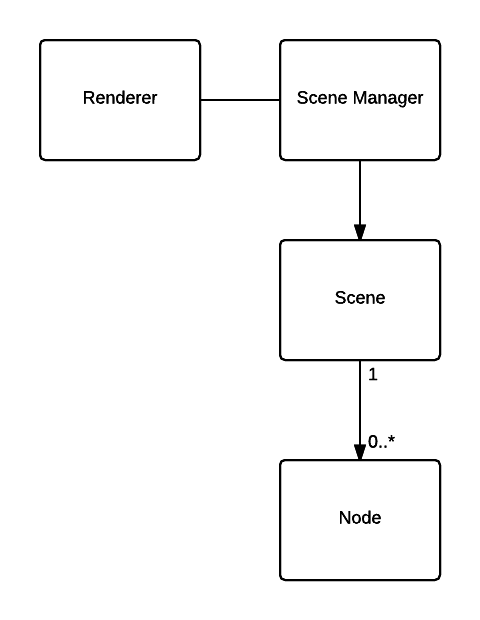
\includegraphics[width=0.6\textwidth]{03-architecture-scene-graph}
%   \caption{Interaction of scene graph components.}
%   \label{fig:scene-graph}
% \end{figure}

% {\brickify} decomposes its features into \class{Plugins}. A
% \class{Plugin} provides a set of methods which can be called upon
% emitted system events to interact with the WebGL scene.
% \citeauthor{brickify-thesis} refers to these callbacks as
% \class{PluginHooks} or just hooks.

% \note{what is a bundle doing here, better intro}
% User interfaces are implemented within the same code package. This
% does not separate the web-interface from the scene features. Thus, it
% is hard to observe and apply changes to the system. The
% interface code uses a \class{Bundle} as an entry point to the plugin
% and scene system. The \class{Bundle} starts \class{Plugins} and loads
% {\threedmodels} from the filesystem into the application.

% {\brickify} provides abstractions for scene management and rendering.
% Plugins interact with the internal system via hooks. The separation of
% {\lego}-conversion features from the rendering engine bring clear
% interfaces. We encountered several hick-ups with this architecture
% when we tried to organize the communication between several plugins.
% In the following sections, we outline our improvements to the internal
% system of {\brickify}. In Section~\ref{sec:reuses-brickify} we talk
% about components which could be reused with minor adaptions.
% Section~\ref{sec:plugin-system} presents the necessary changes to the
% plugin system.

% \subsection{The Framework Reuses Ideas and Components of Brickify}
% \label{sec:reuses-brickify}

% {\brickify} provides a set of core feature any WebGL application can
% make use of. This includes components like the render loop, scene
% management and plugin loading. {\convertify} has the goal to provide
% these essential components to help implementing WebGL application
% fast-forwardly. The implementation of such applications should be
% independent from any user interface code or required frontend
% libraries, avoiding additional vendor-locks to {\threejs}. In this
% section we explain, how we reached this goal.

% \myNotes{work on that section}
% re-uses render loop, scene management, plugin loading, bundle

% changes were: in project structure and ui code <> lots of mixing with
% ui code (convertify does not have any ui code out of the box. that
% will be part of the application that uses convertify)

% To make {\convertify} a multi-purpose WebGL framework, we stripped
% away any interwoven interface code from the \class{Renderer},
% \class{SceneManager} and \class{Bundle}. We also used the plugin
% system of {\brickify}. The applied changes to the plugin system are
% described in the following section.

\subsection{{\convertify} Provides a Plugin System}
\label{sec:plugin-system}

% - Subsection overview

In this section, we present a plugin system that reacts to
{\convertify}'s system events. Additionally, we present a
method, which organizes communication between
\class{Plugins}.

% - Plugin definition in Convertify
% - *feature for web gl scene and reaction on changes of the scene*
% - *full fledged applications will implement a set of plugins to
% provide functionality and web-ui code to provide interface*

A \class{Plugin} bundles an exchangeable set of features
which will interact with the WebGL scene or will react on
changes to the scene. Such features are touch interactions
with the rendered model or computation on the model data
when a \class{Node} is added to the scene. Any full fledged
application implements a set of \class{Plugins} to provide
the scene functionality. E.g. a concrete conversion strategy
provided by {\platener} is implemented by a single
\class{Plugin}.

\subsubsection{Plugins Interact with the Internal System via
  Lifecycle Events}

% - needs-ref :: Lifecycle events in Convertify (= PluginHooks of
% Brickify, Convertify vs. Plugins)
% - needs-figure :: Example Plugin, interacting via PluginHooks
% - System dispatches events (where do events come from?)

{\convertify} emits system events from internal components.
Figure \ref{fig:lifecycle} depicts the system's lifecycle
and the emitted events. The subscribers to system events are
\class{Plugins}. Each event can be handled by a
\class{PluginHook}, if a \class{Plugin} implements it. To
implement a \class{PluginHook} each \class{Plugin} registers
a callback for that event. These callbacks get called when
the event is dispatched by the system. Thus, \class{Plugins}
can react to each event and apply their own functionality to
the scene or even the model geometry. With this we emphasize
compact computation units in plugins, which can still
interact freely with the system.

To better illustrate the work flow of plugins, we have a
short look at an example plugin. The \name{PlatenerPipeline}
plugin is a \class{Plugin} implemented in {\platener}. The
\class{Plugin} reads the model data from a \class{Node}
after a {\threedmodel} was loaded into the scene. Then it
processes the data to create a {\lasercutter} conversion.
When the model is deleted from the scene by a user, the
plugin releases the processed data. This plugin does not
react to further user interactions, like clicking or
rotating the model. Figure \ref{} \myNotes{plugin example
  flow} shows how this plugin integrates with {\convertify}.

\subsubsection{Organizing Plugin Communication with a
  Dispatcher}

% - needs-ref :: mediator organizes communication
% - needs-figure :: mediator between dispatched system events and
%                   plugins (internal handling of system events
%                   before reaching plugins)

As {\convertify} manages multiple plugins, which either
represent computation logic or render components, we have to
know exactly when each of these plugins will interact with the
system. We propose a \class{Dispatcher} component, behaving
similar to the \name{mediator} pattern.

According to \citeauthor{gof}, the \name{mediator} pattern is a
behavioral software design pattern. The mediator encapsulates
interconnections of components. It acts as a communication hub and
coordinates its clients. The client components are loosely coupled as
the clients communicate with the mediator instead of communicating
with each other directly. With a mediator we can model many-to-many
relationships \cite[p. ?]{gof}.\note{fix citing, lookup page}.
% https://sourcemaking.com/design_patterns/mediator

The \class{Dispatcher} implements every \class{PluginHook}.
All system events are emitted to the \class{Dispatcher}
first, before the \class{Dispatcher} will remit them to the
\class{Plugins}. In our case the \class{Dispatcher} is the
mediator, where as the \class{Plugins} are the mediator's
clients. With this component in the middle, we can control
the order in which the events will be received by the
\class{Plugins}. We have to determine the order of
\class{PluginHook} executions explicitly, because for
different events, different \class{Plugins} have to run
first. E.g. {\platener} wants to process the model data
before it is rendered when a user adds a node to the scene.
But it wants to destroy the visualization before releasing
all the computed data. We cannot solve this problem, by
dispatching all events to all plugins in the same order.

To model many-to-many relationships between \class{Plugins}
and \class{Plugins}, we enhance the \class{Dispatcher} with
\class{Protocols}. \class{Protocols} define mixins on the
\class{Dispatcher} which allow delegation of functionality
from the \class{Dispatcher} to a \class{Plugin}. A mixin
adds functionality to an object by object
composition\cite{}\note{give a reference for mixins}. The
delegation pattern achieves the results of multiple
inheritance by object composition. The delegation pattern
speaks of delegating objects and delegates. A delegating
object calls external functionality on a delegate object,
which is available through a predefined interface
\cite{delegation}\note{source for delegation}. In our case,
the \class{Dispatcher} is the delegating object and the
\class{Plugin} is the delegate. The \class{Protocol} helps
to define the interface between the \class{Dispatcher} and a
\class{Plugin}. Two \class{Plugins} now communicate with
each other via the \class{Dispatcher}. One \class{Plugin}
calls functionality on the \class{Dispatcher} which was
exposed by a \class{Protocol}. The \class{Protocol} ensures
that the \class{Dispatcher} delegates an action to another
\class{Plugin}. Figure~\ref{}\note{figure plugin
  communication} shows how the mediator connects two
\class{Plugins}.
% http://best-practice-software-engineering.ifs.tuwien.ac.at/patterns/delegation.html
% https://developer.apple.com/library/ios/documentation/General/Conceptual/DevPedia-CocoaCore/Delegation.html

When applications grow, it is hard to observe all messaging between
components at once. With the \class{Dispatcher}, we wire up all
communication with \class{Plugins} at one place. Due to explicit
ordering of callback executions, we have fine-grained control for each
\class{Plugin}. \class{Protocols} define clean interfaces for
inter-\class{Plugin} communication.

% Each application implemented with
% the {\convertify} framework has to implement a custom
% \class{Dispatcher}.

% - *full fledged applications will implement a mediator to organize
% feature communication*

\section{Platener Is Implemented In {\convertify}}
\label{sec:application-platener}

 % - Section overview
 % - Application is built with Convertify (integration with lifecycle events
 %   and rendering engine)
 % - needs-figure :: Application is separated into Packages
 % - Plugins provide scene feature
 % - Client Code to integrate plugins, system and user interfaces

{\platener} is a web-application, that converts 3D-printable
models into laser-cuttable equivalents. This section
describes the implementation of {\platener} within the
{\convertify} framework. Therefore, {\platener} integrates
with the system events and rendering engine of
{\convertify}. As proposed in the preceding section, it uses
several \class{Plugins} to bring its features to the WebGL
scene. Section~\ref{sec:platener-uses-plugins} describes
these plugins briefly.
Section~\ref{sec:platener-pipeline-plugin} shows
architectural details to the most important \class{Plugin}:
the \name{PlatenerPipeline} plugin. This \class{Plugin}
implements different conversion strategies for
{\threedmodel}s. In Section~\ref{sec:client-to-application}
we explain how the application combines user interfaces with
the \class{Dispatcher} and the \class{Plugins}.

\subsection{Platener Uses Plugins to Implement Its Features}
\label{sec:platener-uses-plugins}

The \class{Plugins} composed into {\platener} provide its
computation logic and WebgGL scene rendering. We will give a
brief introduction of each plugin in the following
paragraphs.

\subsubsection{Platener Pipeline Plugin}

The \name{PlatenerPipeline} plugin does the major work on
converting {\threedmodels} to 2D-plates. The plugin defines
multiple conversion approaches. A conversion is an
approximation of the original model with plates.
Figure~\ref{fig:conversion:plate} and
Figure~\ref{fig:conversion:stacked} show two conversion
results. This plugin generates a set of 2D-paths, so that
the conversion can be produced with a {\lasercutter}. The
paths are depicted in Figure~\ref{fig:conversion:paths}.
Section~\ref{sec:platener-pipeline-plugin} explains the
architecture of the \name{PlatenerPipeline} plugin in
detail.

\begin{figure}[h]
  \centering
  \begin{subfigure}[a]{0.3222\textwidth}
    \includegraphics[width=\textwidth]{}
    \caption{A box converted with hull approximation.}
    \label{fig:conversion:plate}
  \end{subfigure}
  \begin{subfigure}[b]{0.3222\textwidth}
    \includegraphics[width=\textwidth]{}
    \caption{A box converted with stacked approximation.}
    \label{fig:conversion:stacked}
  \end{subfigure}
  \begin{subfigure}[c]{0.3222\textwidth}
    \includegraphics[width=\textwidth]{}
    \caption{2D-paths of the box converted with hull approximation.}
    \label{fig:conversion:paths}
  \end{subfigure}
  \caption{Results of the \name{PlatenerPipeline} plugin.}
  \label{fig:conversion}
\end{figure}

% The \name{PlatenerPipeline} plugin is the main computation unit.
% The \class{Plugin} defines multiple {\fabmethod}s. A
% {\fabmethod} is a conversion approach of a \threedmodel.
% Multiple computation steps, which can manipulate the input
% model, are chained after another to produce 2D- or
% 3D-output. For example, construction plans in the format of
% {\svgfile}s are such an output, see Figure~\ref{}
% \note{construction plans figure}.
% Section~\ref{sec:platener-pipeline-plugin} explains the
% architecture of the \name{PlatenerPipeline} plugin in detail.

\subsubsection{Node Visualizer Plugin}

We visualize the results of the \name{PlatenerPipeline}
plugin in the WebGL view. The \name{NodeVisualizer} plugin
renders the results of each conversion and its intermediate
computation steps respectively. With the help of this we
debug the results of the computation visually. As explained
in Section~\ref{}\note{section walkthrough}, we select a
single visualization at a time to inspect the results of the
step associated with the visualization.
Figure~\ref{fig:steps:plate} shows a head-mounted display in
the \name{Plate} step. Figure~\ref{fig:steps:ui} shows the
selection of that visualization in the user interface.

\begin{figure}[h]
  \centering
  \begin{subfigure}[a]{0.48\textwidth}
    \includegraphics[width=\textwidth]{}
    \caption{A head-mounted display, consisting of plates only.}
    \label{fig:steps:plate}
  \end{subfigure}
  \begin{subfigure}[b]{0.48\textwidth}
    \includegraphics[width=\textwidth]{}
    \caption{The selection of the intermediate plate step in
      the user interface.}
    \label{fig:steps:ui}
  \end{subfigure}
  \label{fig:steps}
  \caption{Visual debugging of intermediate conversion results.}
\end{figure}

\subsubsection{Scorer Plugin}

We run multiple conversion approaches sequentially. Then, we choose
the best fitted conversion as output. Thus each conversion
is scored by a scoring algorithm. This
\clas{Plugin} provides such scoring algorithms.

\subsubsection{Solution Selection Plugin}

This plugin utilizes the \name{Platener Pipeline} plugin and
the \name{Scorer} plugin to run and evaluate all conversion
approaches. It outputs the result of the conversion with the
best score.

\subsubsection{Coordinate System Plugin}

This plugin provides orientation enhancements for the WebGL
scene. Rendering xyz-axes and a an axis-aligned grid, users
can grasp alignment and dimensions of {\threedmodel}s.
Figure \ref{fig:architecture_overview_coordinate_system}
shows the coordinate system in the WebGL view. The
Coordinate System is taken from \emph{Brickify} as
is\cite{}\note{ref chapter in brickify}.

\begin{figure}
  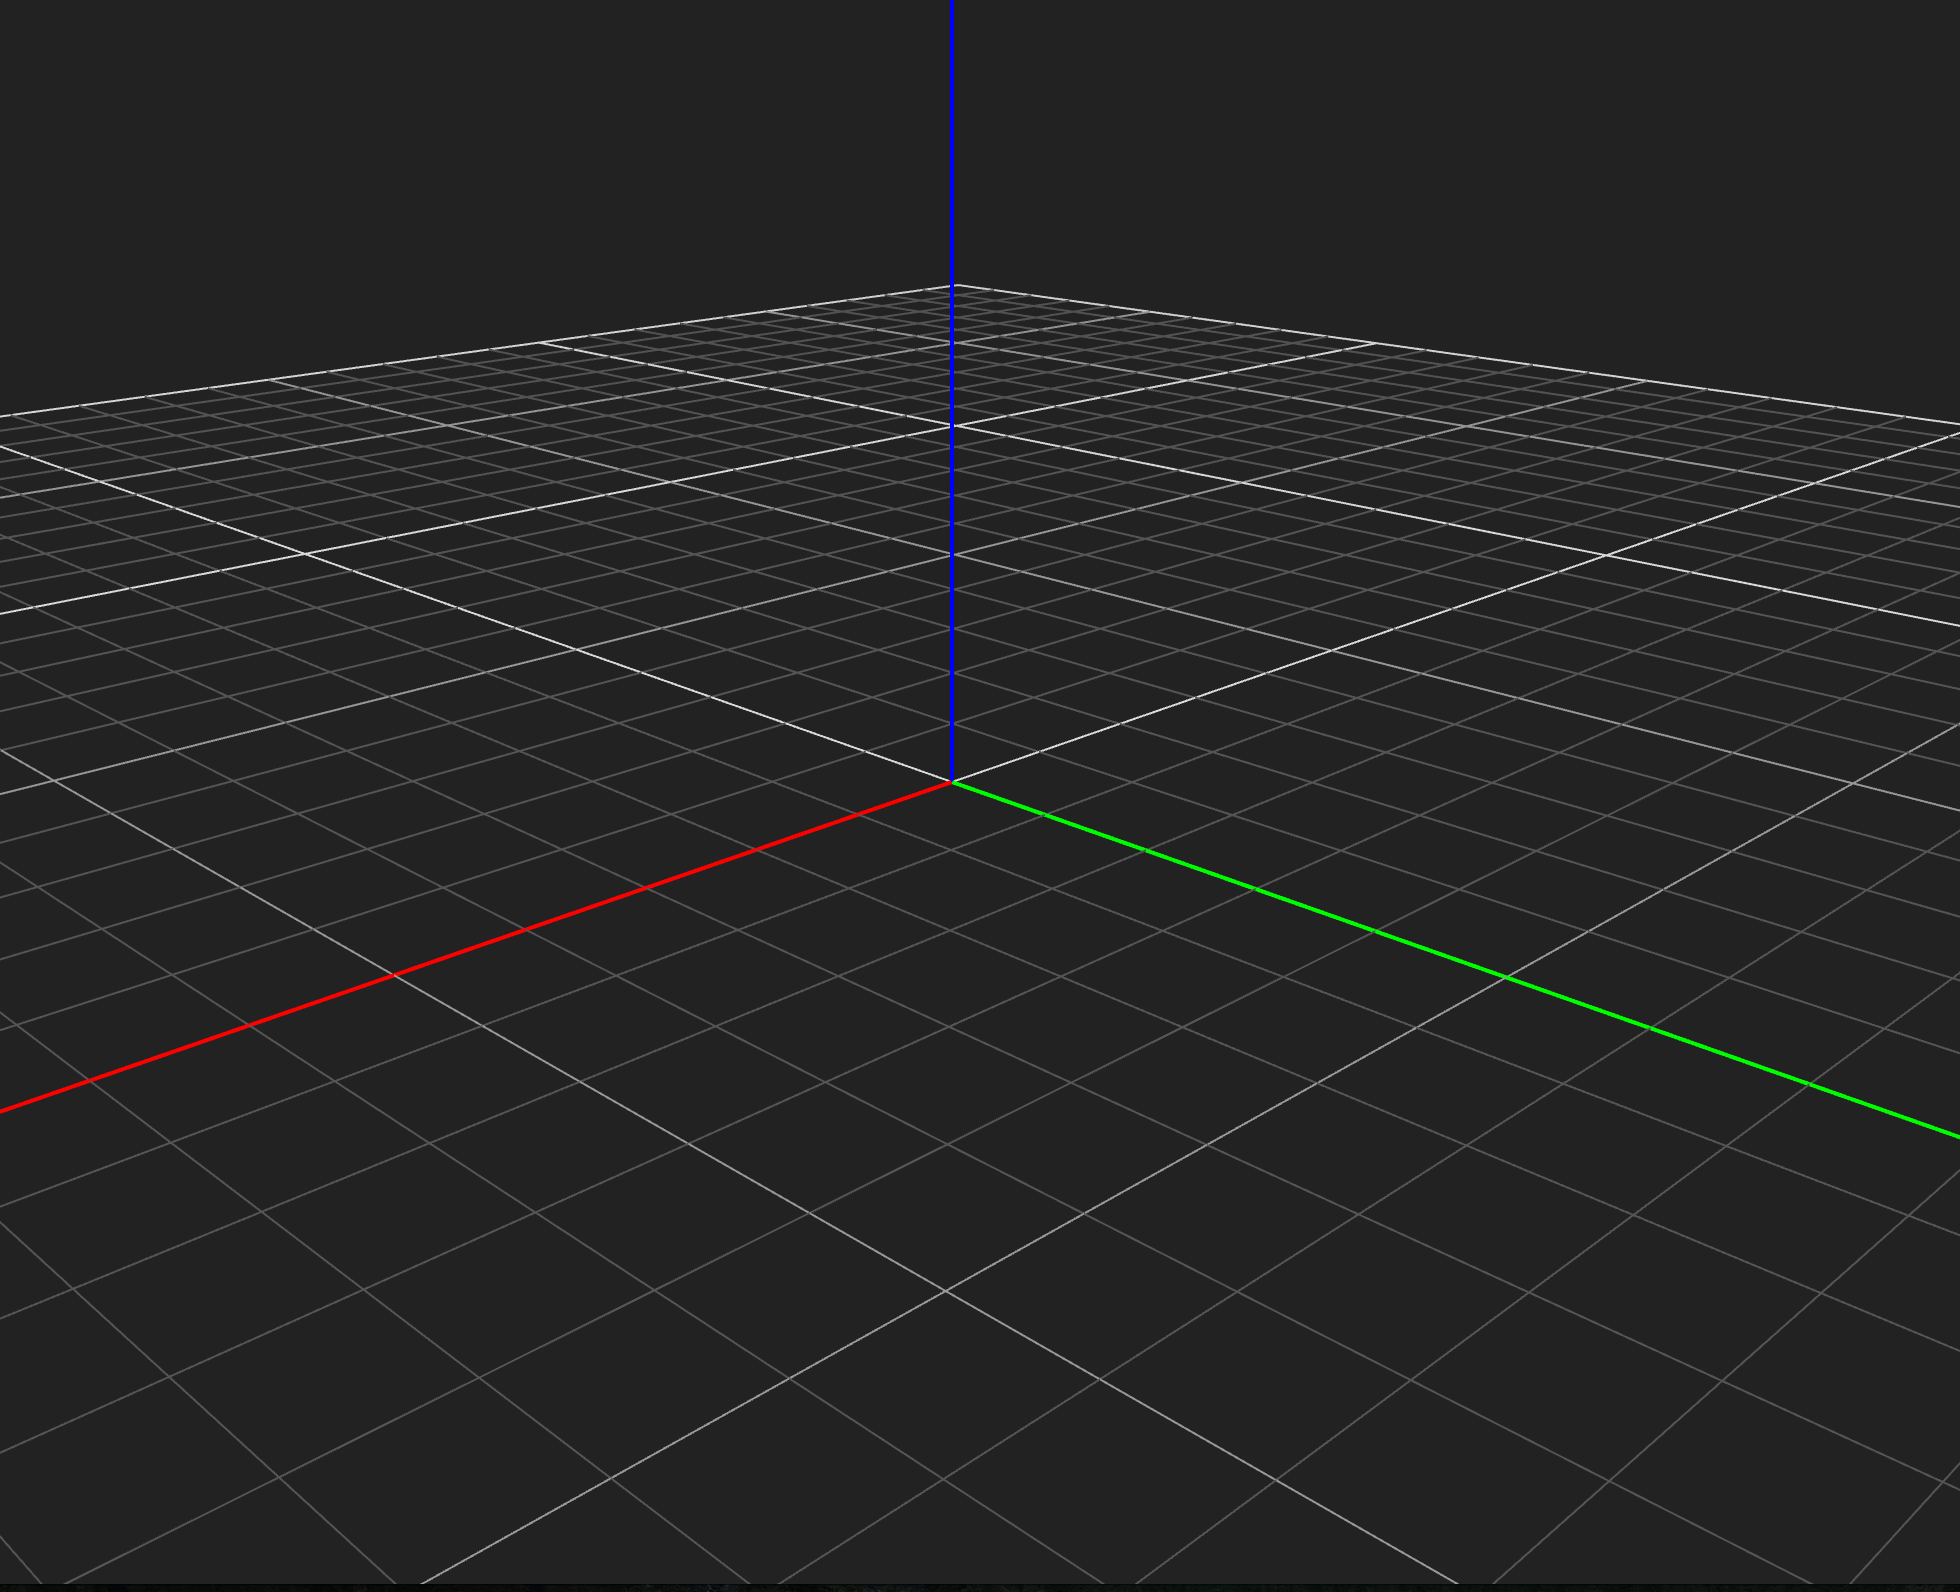
\includegraphics[width=1\columnwidth]{03-architecture_overview_coordinate_system}
  \caption{An empty scene showing the coordinate system.}
  \label{fig:architecture_overview_coordinate_system}
\end{figure}

\subsubsection{Isolated Testing Plugin}

While we developed on different stages of a sequentially
executed conversion approach in parallel, we needed a
mechanism to test each component of the conversion before
its preceeding or succeeding components were completely
implemented. The \name{IsolatedTesting} plugin provides an
isolated environment, which allows to execute a single
intermediate computation step of a conversion approach with
pre-defined input.

\subsection{The PlatenerPipeline Plugin Computes the Model
  Conversions}
\label{sec:platener-pipeline-plugin}

% - Subsection overview

The \name{PlatenerPipeline} is the main computation unit of
{\platener}. It contains algorithms and data structures to
bring the {\threedmodel} into a 2D-representation suitable
for a {\lasercutter}. In this section we dive into details
about the computation process. First we look at
{\platener}'s three conversion approaches. Then, we explain
the composition of conversion approaches from computation
steps into a \class{Pipeline} data structure. Finally, we
present the \class{PipelineState}, a data structure which
allows to take a snapshot of the computation state in
between two computation steps. The \class{PipelineState} is
used to render the visualizations of the
\name{NodeVisualizer} plugin.

% - needs-figure :: Pipelining Approach to subdivide the problem space
% - PipelineSteps as single computation units
% - Several Pipeline Steps make up a Fabrication Method

\subsubsection{{\platener} Presents Three Conversion
  Approaches}

The \name{PlatenerPipeline} plugin facilitates conversion
approaches. We call such a conversion approach
\class{\fabmethod}.
%A {\fabmethod} is a conversion approach of a {\threedmodel}.
It defines a linear process of analyzing a {\threedmodel}
and thereby creates a suitable equivalent of the model,
consisting of plates only. A \class{\fabrication} method
divides the conversion problem into smaller problems. Thus,
it provides a set of algorithms, which are executed
sequentially. Each algorithm solves a single subproblem. The
algorithms work on results of previously executed
algorithms. We refer to a sequence of algorithms as
\class{Pipeline}. Each algorithm in the \class{Pipeline} is
an intermediate computation step, called
\class{PipelineStep}. The first \class{PipelineStep} works
on the face-vertex-mesh of the model. The last
\class{PipelineStep} returns a directly exportable data
format, in our case a {\zipfile} containing the
2D-construction plans. The composition of
\clas{PipelineSteps} into a \class{Pipeline} is shown in
Figure~\ref{fig:pipeline-from-steps}. \class{PipelineSteps}
are independent from the \class{\fabmethod} and thus, can be
shared between different \class{{\fabmethod}s}. {\platener}
provides three \class{{\fabmethod}s}. The following paragraphs
present each method briefly.

\begin{figure}[h]
\centering
\begin{verbatim}
- show multiple pipeline steps with inlets/ outlets of
pipeline state
- make clear, that a pipeline step is an algorithm, solving
a sub problem
- pipeline like a swimming lane, where pipeline steps
connect
- a model comes in
- a construction plan falls out (zip file)
\end{verbatim}
\caption{A \class{Pipeline} is composed from
  \class{PipelineSteps}}
\label{fig:pipeline-from-steps}
\end{figure}

\paragraph{Plate Method}

This \class{\fabmethod} does hull and surface
reconstructions of the input model. We produce a set of
plates which are connected via finger joints to approximate
the original {\threedmodel}. Therefore, we first detect the
outlines of all surfaces in the model. Then, we search for
existing plates based on that surfaces. For example two
parallel surfaces form an \name{inherent} plate, when they
are about three to five millimeters apart. After we found
all \name{inherent} plates, we construct plates from the
remaining surfaces by \name{extruding} the planar shapes.
Then we connect the plates with finger joints where they
touch each other. Figure~\ref{fig:model-fingers} shows
plates connected with finger joints.
Figure~\ref{fig:overview-plate-steps} depicts the important
\class{PipelineSteps} of the \name{Plate Method}.
\note{remake this figure with our steps}

\begin{figure}[h]
  \centering
  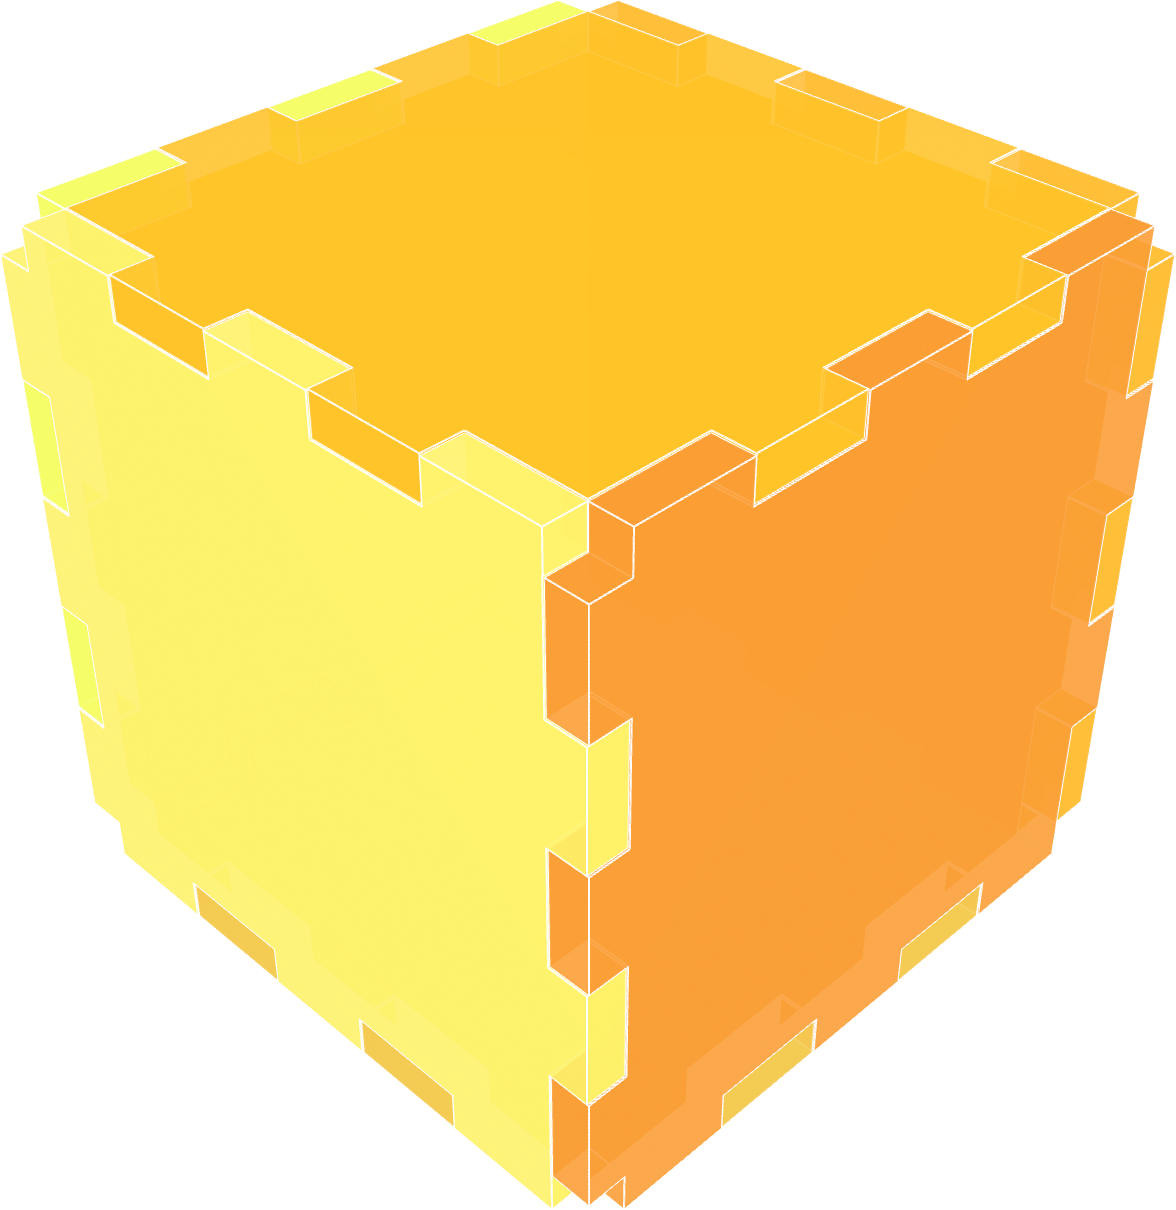
\includegraphics[width=0.6\textwidth]{03-architecture-box-fingers}
  \caption{A model built from plates, connected with finger
    joints.}
  \label{fig:model-fingers}
\end{figure}

\begin{figure}[h]
  \centering
  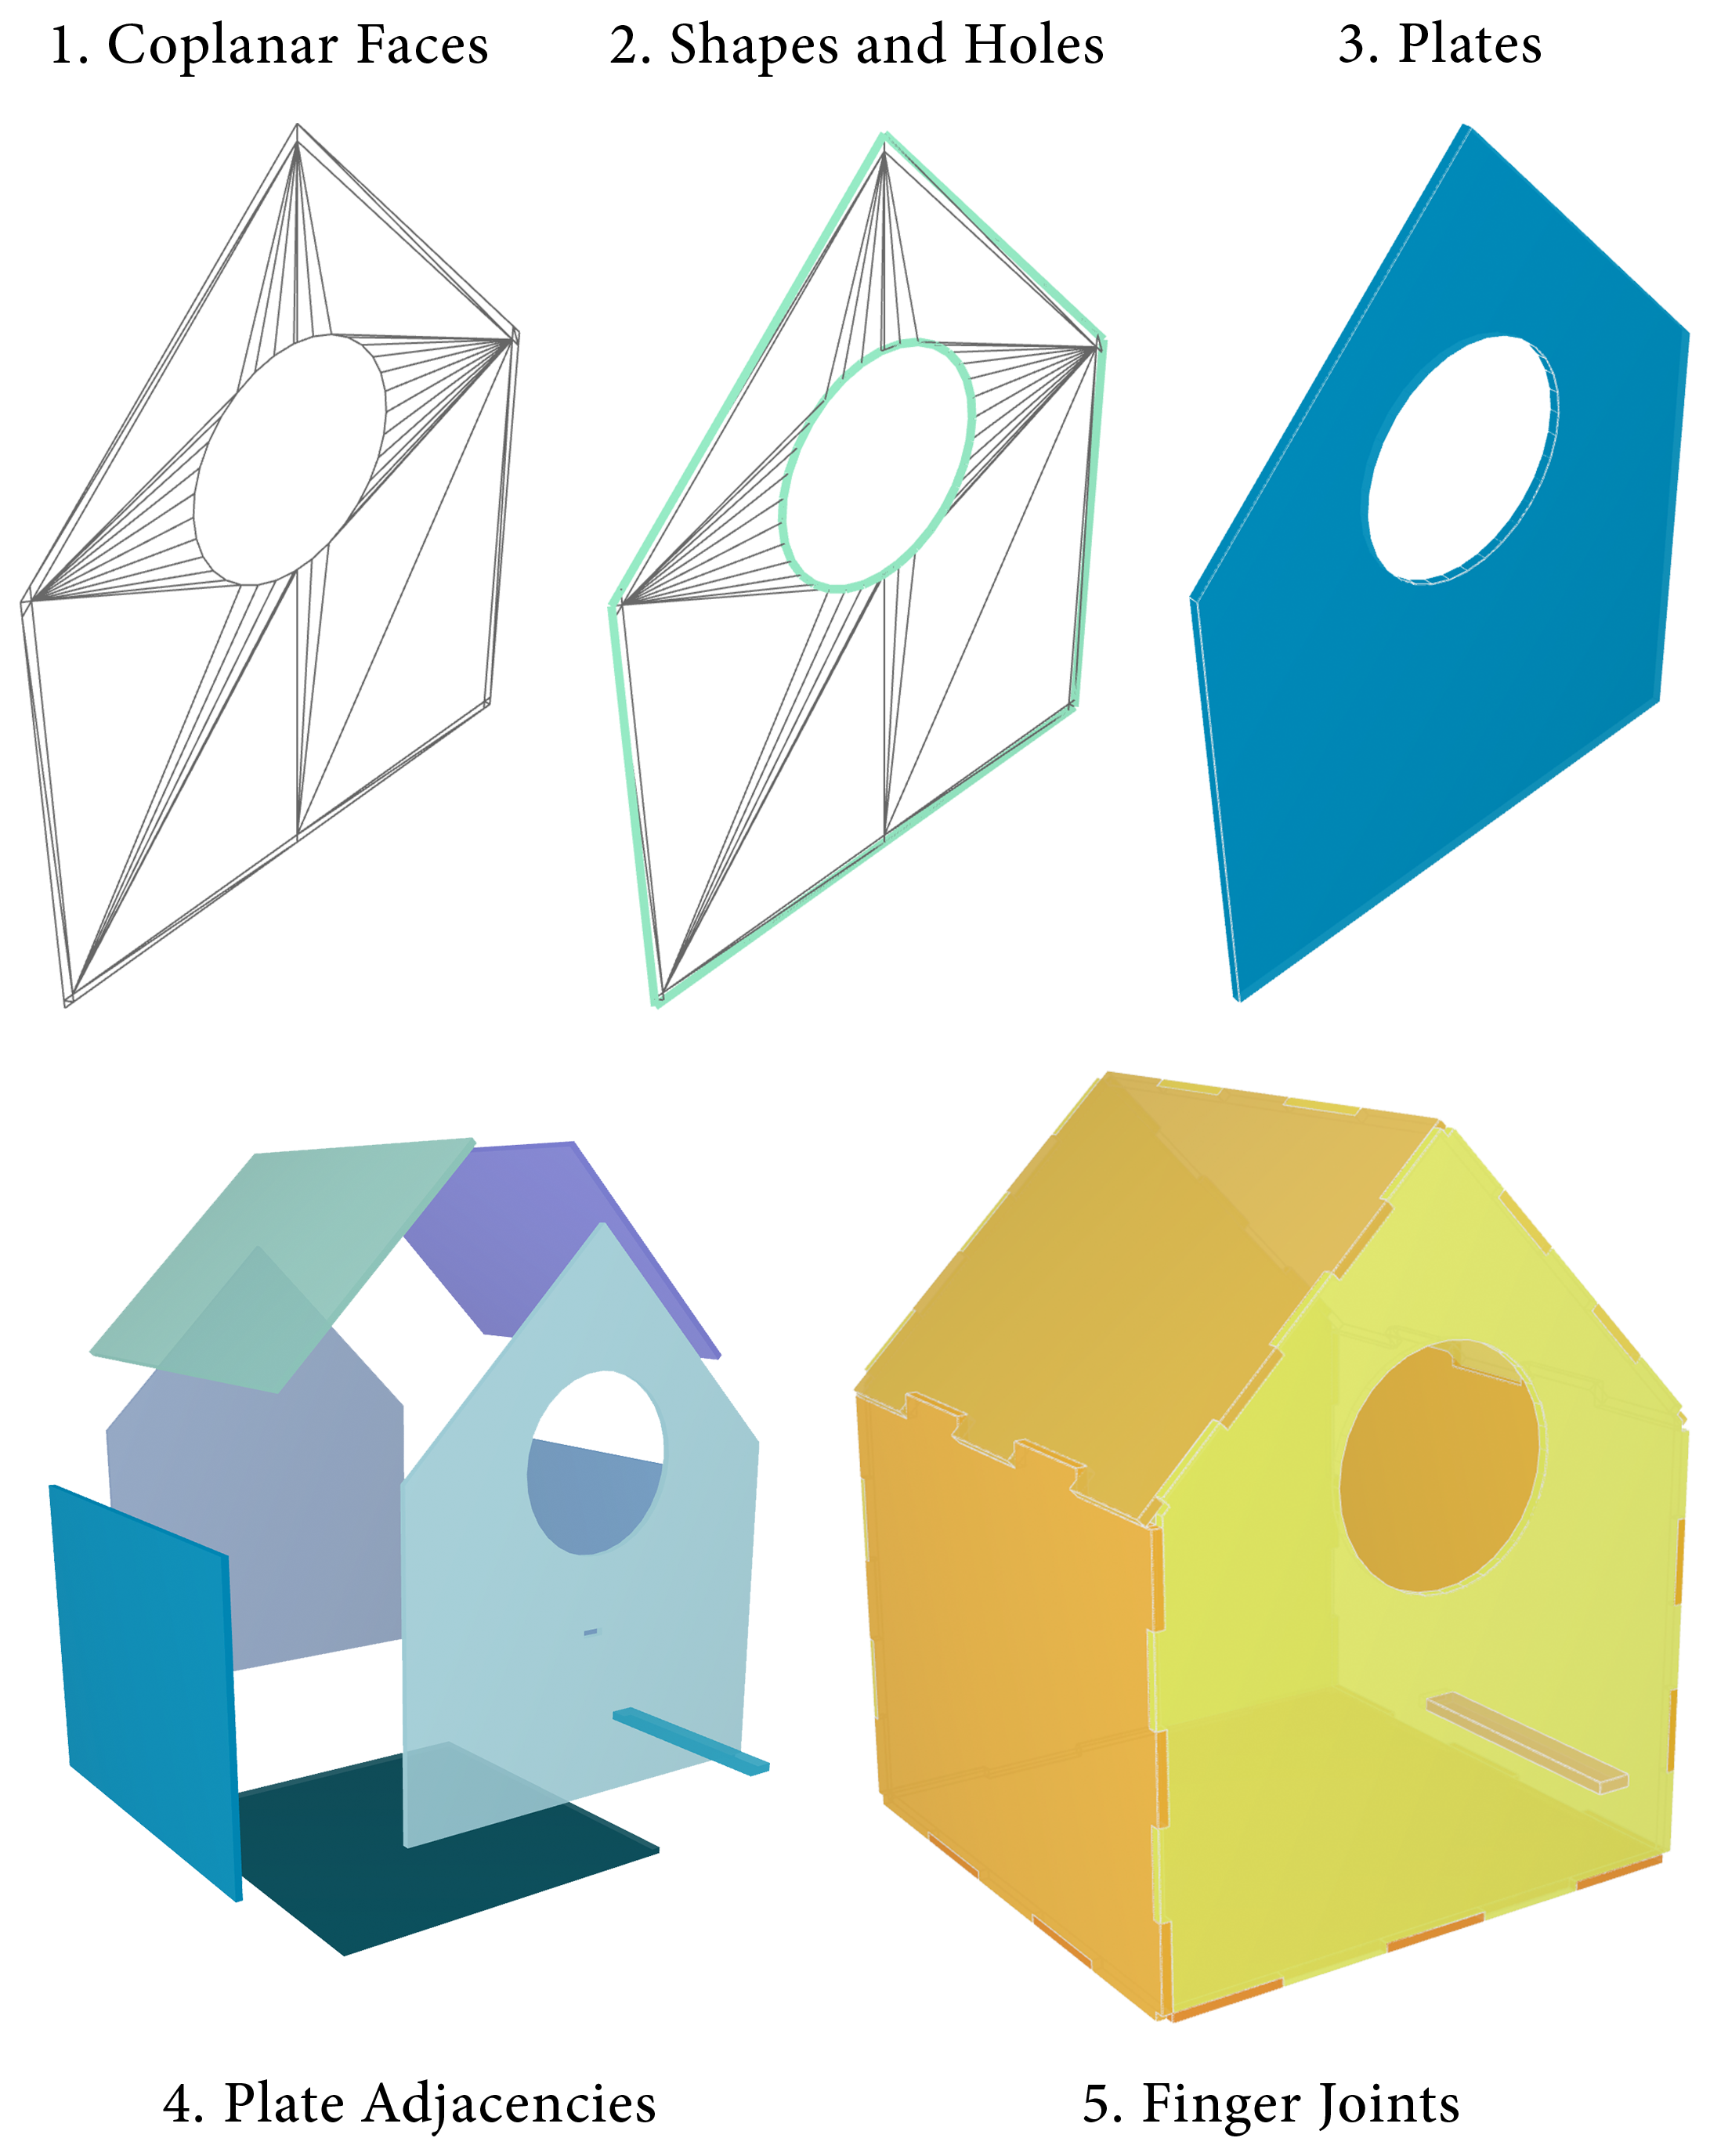
\includegraphics[width=1\textwidth]{03-architecture-pipeline-steps-overview}
  \caption{An overview of computation steps that are applied
    to the model, so that it can be built from plates..}
  \label{fig:overview-plate-steps}
\end{figure}


\note{ref to chapters which explain the algorithms to that
  method in detail}

\paragraph{Stacked Plates Method}

This \class{\fabmethod} does volume reconstructions of the
input model. We stack plates onto each other to approximate
the shape of the original model, see
Figure~\ref{fig:stacked-rabbit}. This preserves the look and
feel of the model. We slice the model into equally thick
layers, which form the plates. The plates are then connected
via shafts to simplify the assembly process.

\begin{figure}[h]
  \centering
  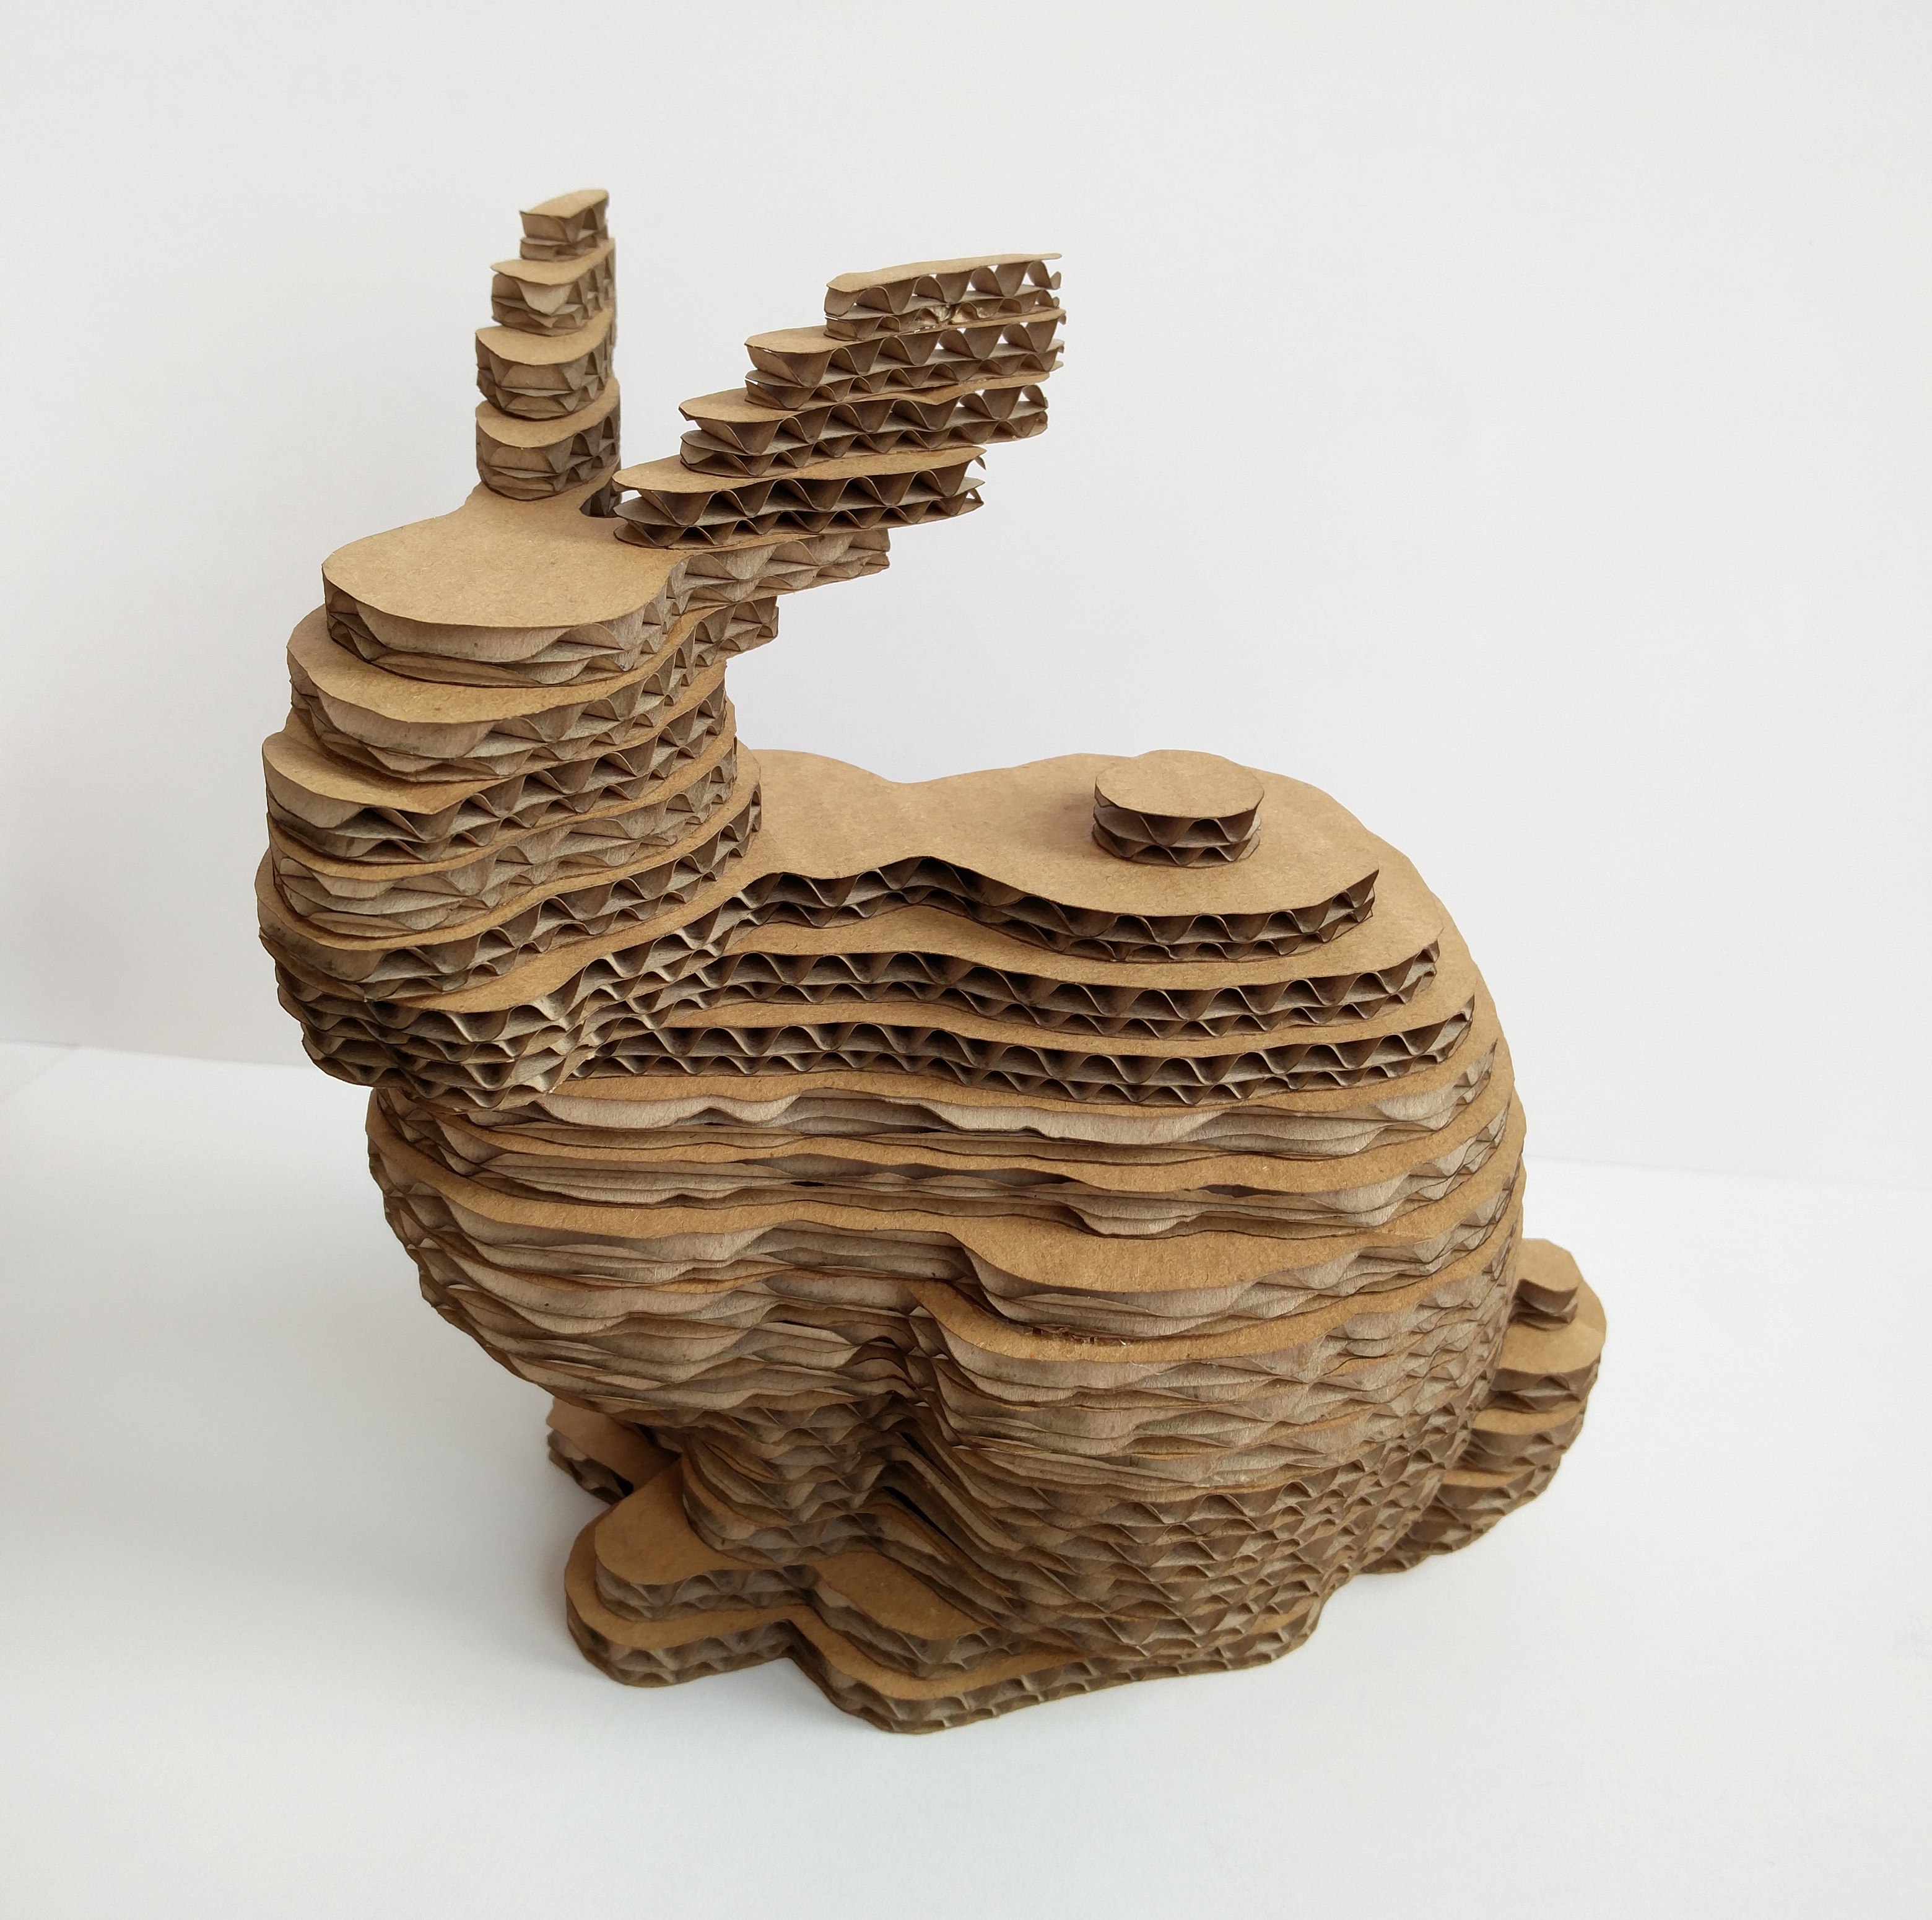
\includegraphics[width=0.6\textwidth]{03-architecture-rabbit-stacked}
  \caption{A rabbit model converted to plates with
    stacking.}
  \label{fig:stacked-rabbit}
\end{figure}
\note{ref to chapters which explain the algorithms to that
  method in detail}

\paragraph{Classifier Method}

This is an advanced conversion approach, combining intense
mesh analysis and sophisticated construction techniques of
known geometries. This \class{\fabmethod} will be more
robust when converting models with noisy mesh data, e.g
{\threedmodel}s with lots of texture on their surface. We
analyze the model for primitive geometries using random
algorithms. Primitive geometries are planes, prisms, boxes,
cylinders or spheres. The model is structured into an
hierarchical graph structure, similar to a scene graph,
consisting of these primitive geometries only. For each of
these primitives we know a conversion approach to plates,
which will then give better results for the conversion of
the whole input model. The \name{Classifier Method} is a
proposal and still work in progress. We can currently
classify a subset of the primitive geometries.
Figure~\ref{fig:tiki-cylinder} shows the classification of a
cylinder in a model. In Chapter~\ref{} \note{ref the
  chapter!} we give details about the random algorithm,
which classifies the primitives.

\begin{figure}[h]
  \centering
  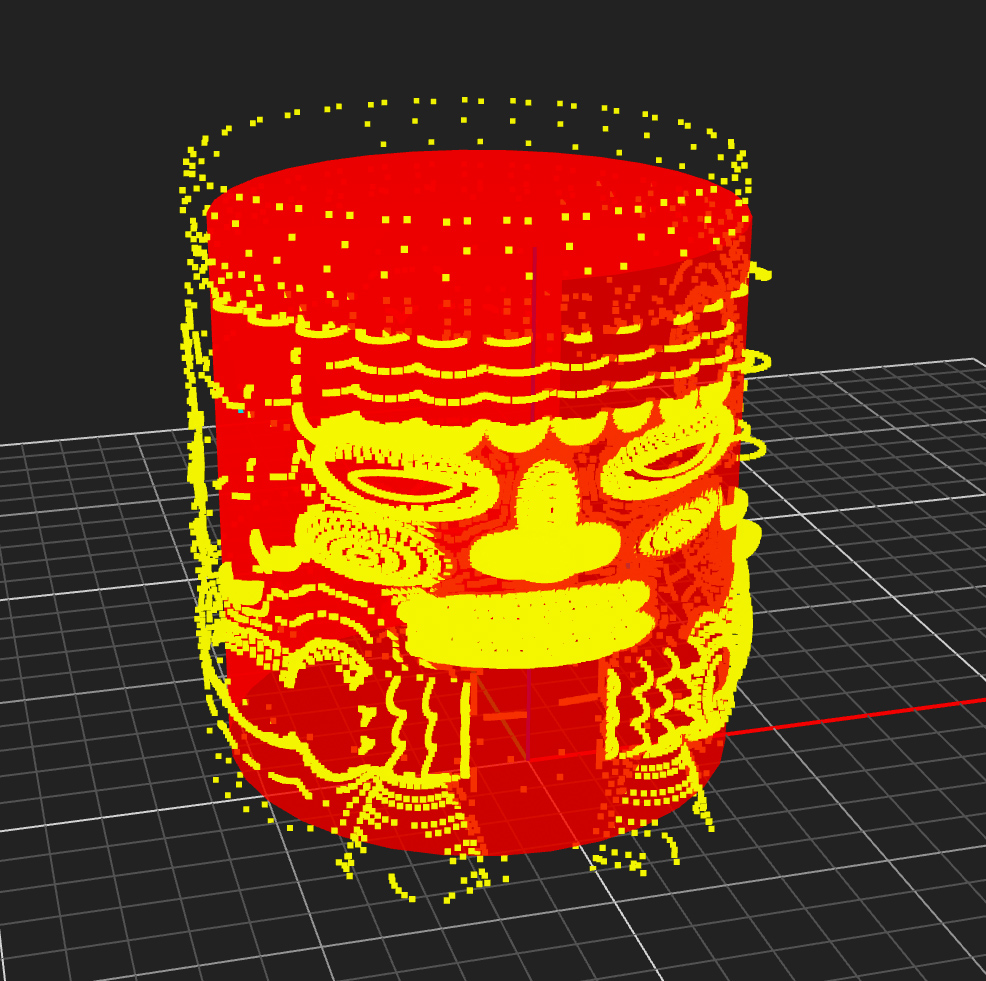
\includegraphics[width=0.6\textwidth]{03-architecture-tiki-cylinder}
  \caption{A classified cylinder in a model with textures.
    The yellow points, show the outline of the actual model.}
  \label{fig:tiki-cylinder}
\end{figure}

\paragraph{}

\note{summary}

\subsubsection{Pipeline Steps Compute Cloneable State}

Each \class{\fabmethod} assembles a \class{Pipeline} from
\class{PipelineSteps}. \class{PipelineSteps} work on the
data of previous computation steps and pass the data to the
next compution steps. To improve the development and
debugging experience, we not only pass the results of the
\class{PipelineStep} to the following step, but we also
preserve a snapshot of the data. We call the state of a
given data structure at a given point in time a snapshot. A
snapshot of the computed data is used to render a visual
representation of the data. The visual representation gives
a clear understanding of the data and thus enhances the
development and debugging experience. In this section we
explain how the \class{Pipeline} takes snapsots of the
results of \class{PipelineSteps}. Note, that the
\class{PipelineSteps} are merely computation units. All
visual output is done in the \name{NodeVisualizer} plugin.

When we take a snapshot of the results of a
\class{PipelineStep}, we ensure, that modifications of a
latter \class{PipelineStep} will not alter the data in the
snapshot of a previous \class{PipelineStep}. Otherwise, the
\name{NodeVisualizer} plugin renders corrupted visuals for
the previous step. Figure~\ref{fig:corrupt} shows how the surface
reconstruction step, which comes early in the
\class{Pipeline}, is effected by the creation of finger
joints.

\begin{figure}[h]
  \centering
  \begin{subfigure}[a]{0.3222\textwidth}
    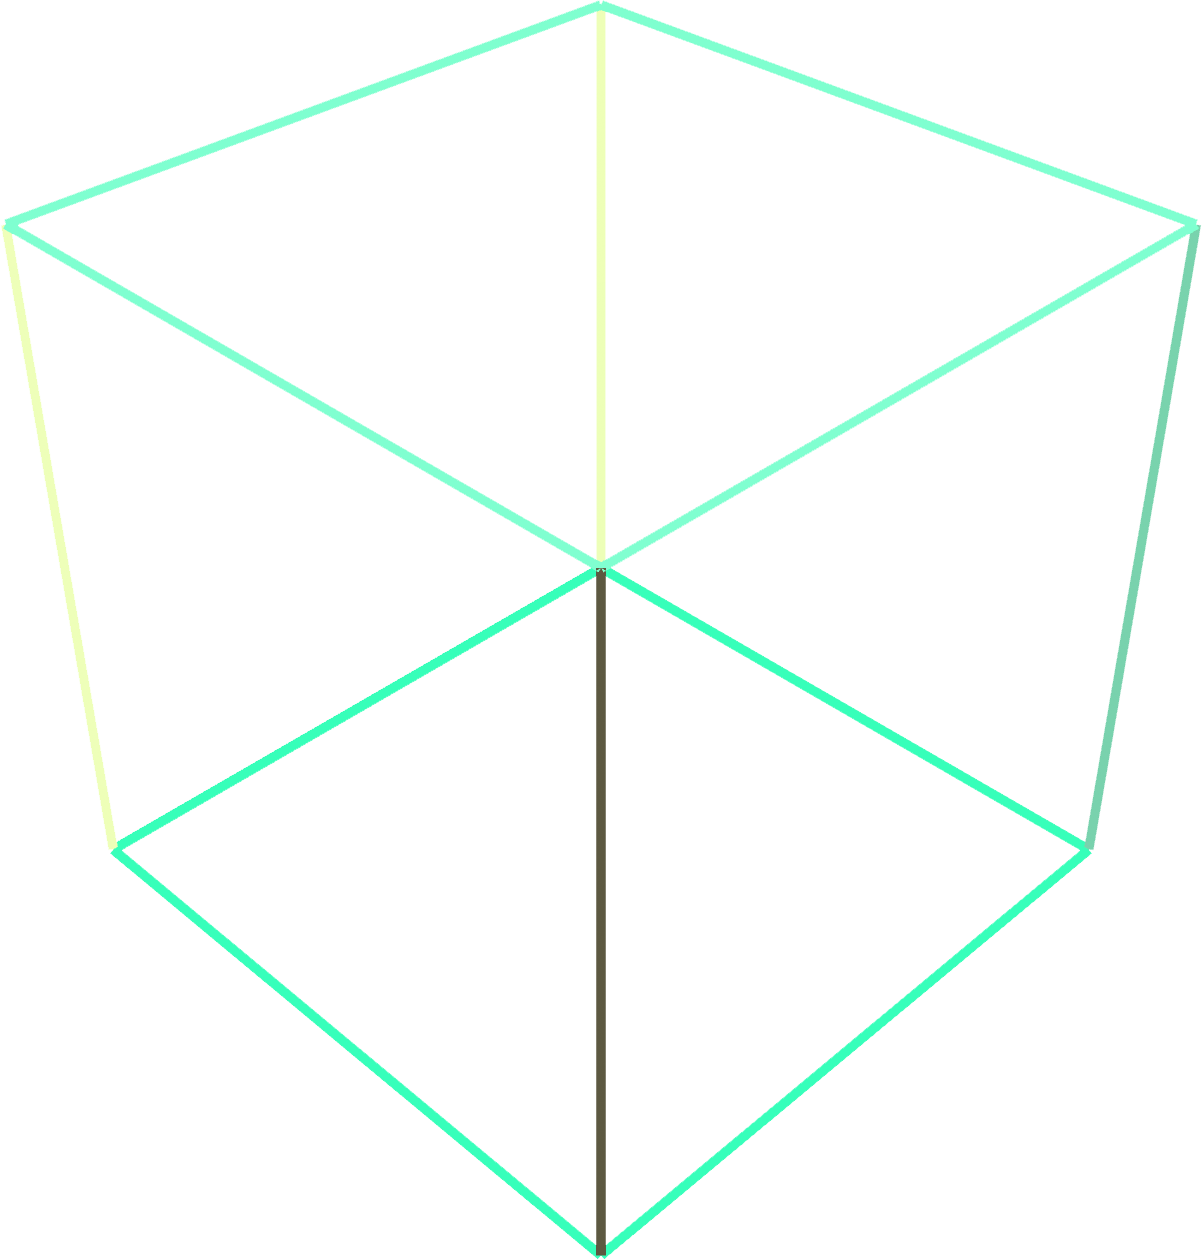
\includegraphics[width=\textwidth]{03-architecture-box-shapes}
    \caption{The shapes of a box.}
    \label{fig:corrupt:shapes}
  \end{subfigure}
  \begin{subfigure}[b]{0.3222\textwidth}
    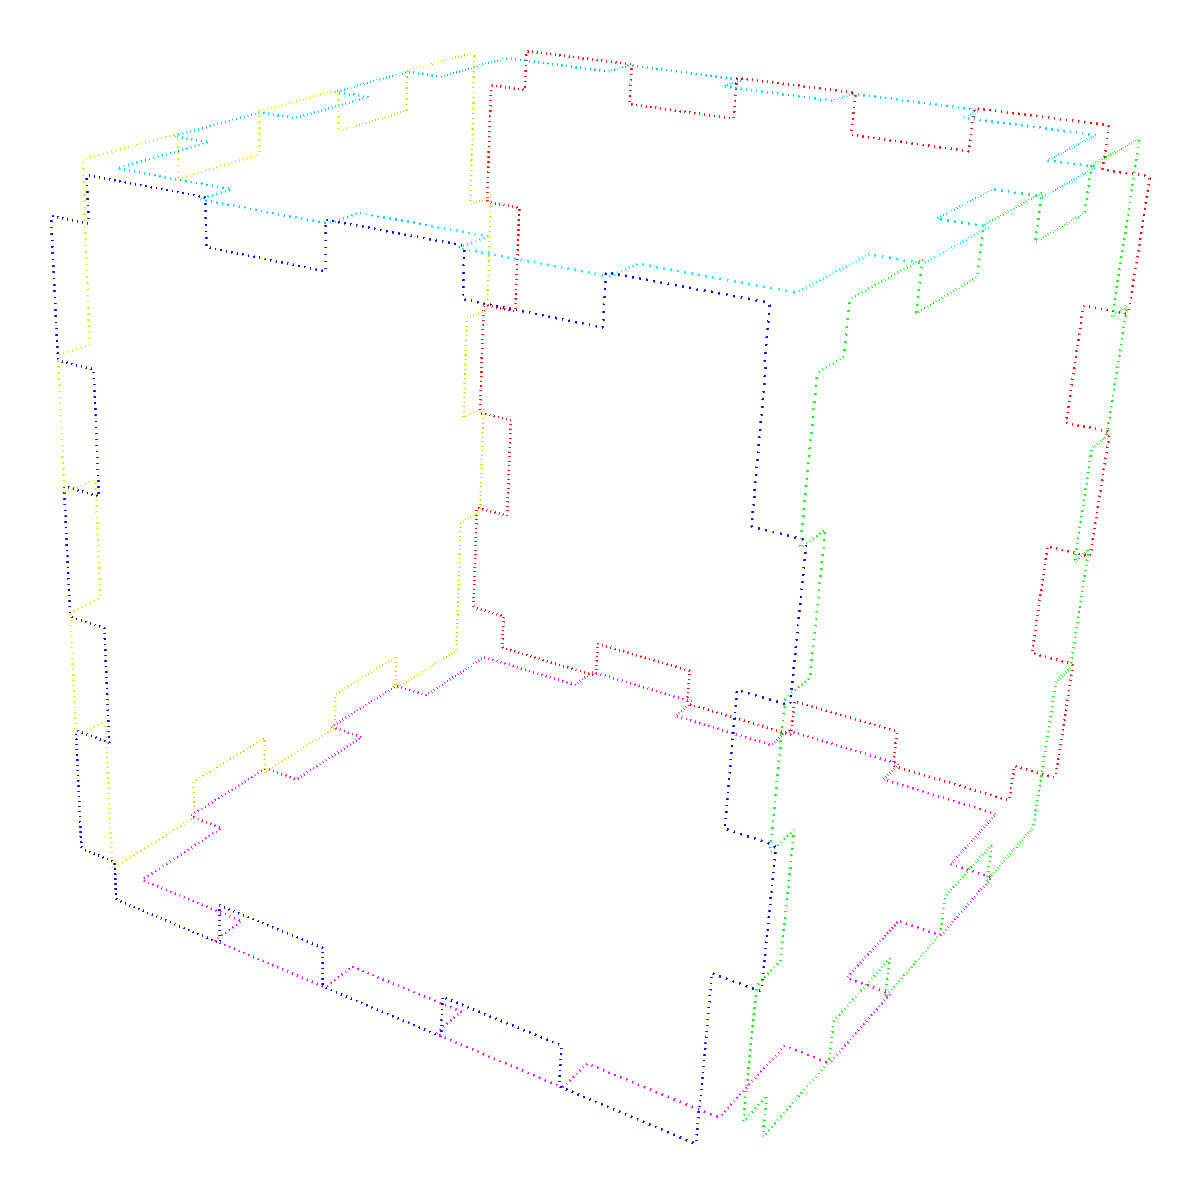
\includegraphics[width=\textwidth]{03-architecture-box-shapes-with-fingers}
    \caption{Corrupted shapes of a box, showing the finger joints.}
    \label{fig:corrupt:shapes-fingers}
  \end{subfigure}
  \begin{subfigure}[c]{0.3222\textwidth}
    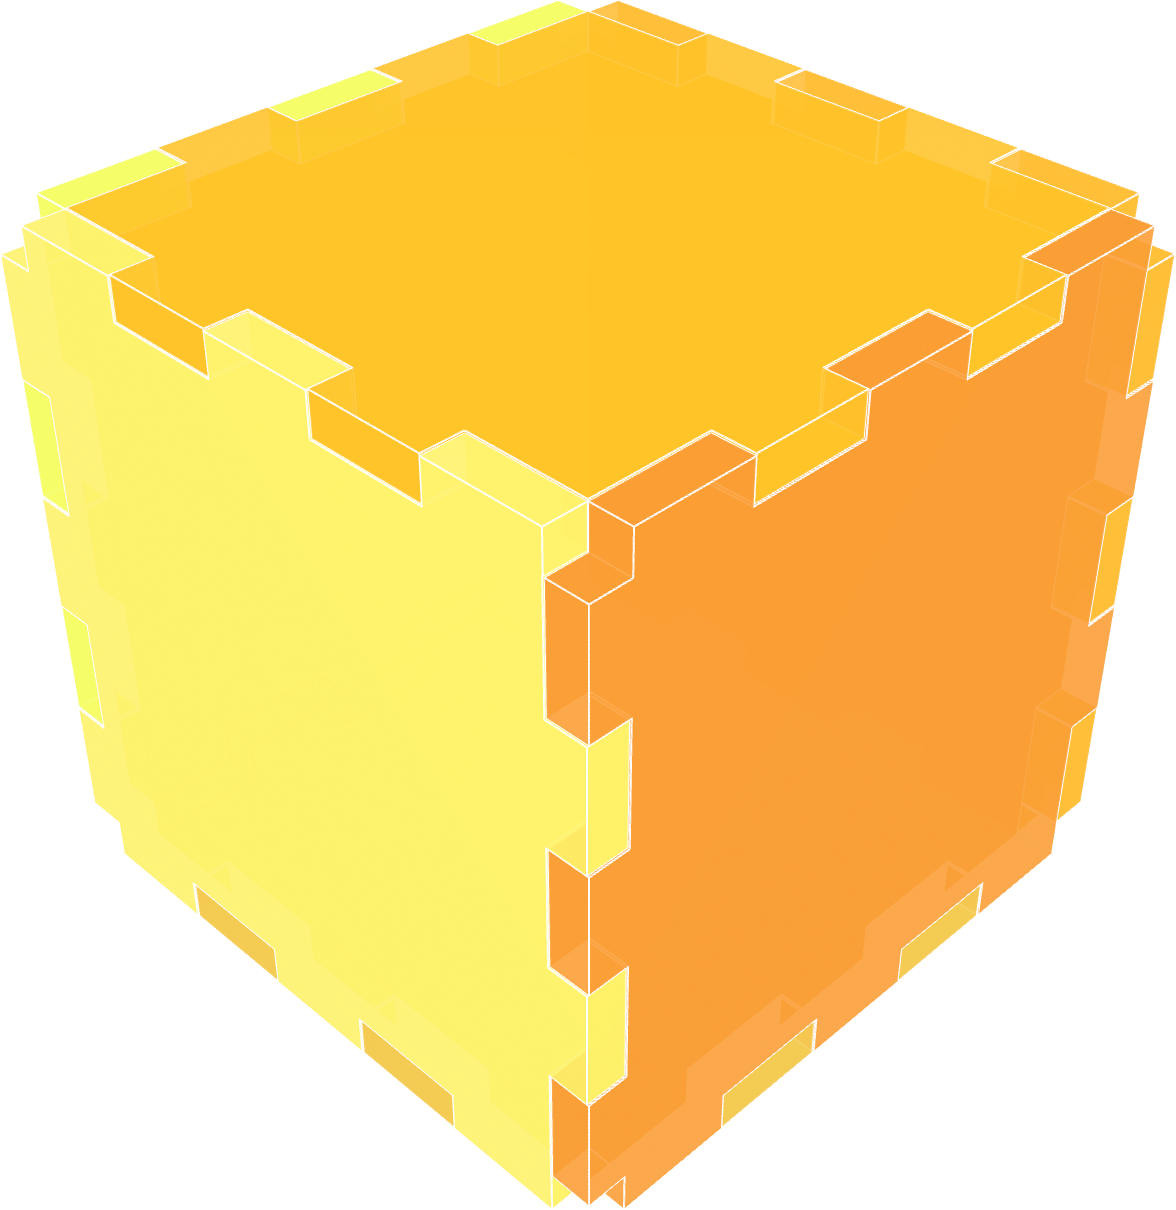
\includegraphics[width=\textwidth]{03-architecture-box-fingers}
    \caption{A box with finger joints.}
    \label{fig:corrupt:fingers}
  \end{subfigure}
  \caption{Modifications to shallow copies of the data
    corrupt the visualizations.}
  \label{fig:corrupt}
\end{figure}

We create deep copies of the data structures, to persist the
data of the snapshots. A deep copy of a data structure, is a
clone of all fields of that data structure. That means if a
data structure references dynamically allocated memory, we
do not clone the reference of the allocated memory to the
copy of the data structure. Instead, we allocate new memory
and duplicate the data to the newly allocated memory. Thus,
we make sure modifications on the copy do not alter the
original. Listing~\ref{lst:deep-copy} shows the effects of a
deep copy.

\begin{listing}[h]
\begin{minted}[
linenos
]{coffeescript}
data = createDynamicMemoryWith('foo')
copy = data.copy()

# both structures have the same copied data
data.dynamicMemory # = foo
copy.dynamicMemory # = foo

# alter the dynamically allocated memory
changeFooToBar(copy.dynamicMemory)

# a shallow copy will effect both,
# the data and the copy
copy.dynamicMemory # = bar
data.dynamicMemory # = bar

# a deep copy prevents this effect
data = createDynamicMemoryWith('foo')
deepCopy = data.deepCopy()

data.dynamicMemory # = foo
copy.dynamicMemory # = foo

changeFooToBar(copy.dynamicMemory)

copy.dynamicMemory # = bar
data.dynamicMemory # = foo
\end{minted}
\caption{A {\coffeescript} example showing the effects of a deep copy
  of data.}
\label{lst:deep-copy}
\end{listing}

% - needs-figure, needs-ref :: Immutable PipelineState
% allows timetravel visual debugging

The data that is passed between the \class{PipelineSteps} is
encapsulated in a \class{PipelineState}. The
\class{PipelineState} contains all data structures that are
ever to be computed by all \class{PipelineSteps}. It is
essentially a container for every computation result.

A snapshot is obtained by cloning the \class{PipelineState}
after the execution of a \class{PipelineStep}. The
\class{PipelineState} is an clonable data structure. A
cloneable data structure can be copied. We provide a deep
copy for the \class{PipelineState}, so that any changes to
the copy will not affect the original and vice-versa.
Figure~\ref{} \note{steps and snapshots flow} illustrates
how snapshots are obtained between two
\class{PipelineSteps}. The encapsulated data in the state
can be hierarchical and complex. We provide a fully
cloneable data structure. That means, any nested data
structure in the \class{PipelineState} implements a
cloneable interface and supports deep copies. Thus, we
ensure that modifications to any nested data by latter
\class{PipelineSteps} do not modify previous copies of the
data.


% \item Pipeline Implementation

%   \begin{enumerate}
%   \item the pipeline works as follows...
%     \begin{itemize}
%     \item Pipeline class
%     \item pipe interface for Step factories (compare listing above, stacked method)
%     \item create state factory -> use composition to persist intermediate results
%       (state is later accessed by node visualizer)
%     \item reduce approach -> pipe last state into next step to produce new state
%     \item show a listing of pseudo code, explaining how the pipeline works
%     \item benchmarking (measure time for intermediate steps vs whole processing)
%     \end{itemize}

%   \item it can be reused (because pipelining is a generic concept)
%     \begin{itemize}
%     \item classifier graph (classification method)
%     \item isolated testing (injectable pipeline)
%     \end{itemize}
%   \end{enumerate}

% \end{enumerate}


\subsection{The Client Package Connects All Features Into an
  Application}
\label{sec:client-to-application}
\note{concrete heading: platener instead of application}

% - Subsection overview

This section describes the code packages of {\platener}.
Furthermore, we explain the how {\convertify} is used by
{\platener} and how the user interface is connected to the
\class{Plugins}.

%     - needs-figure :: Application is separated into
%     Packages


\begin{figure}
  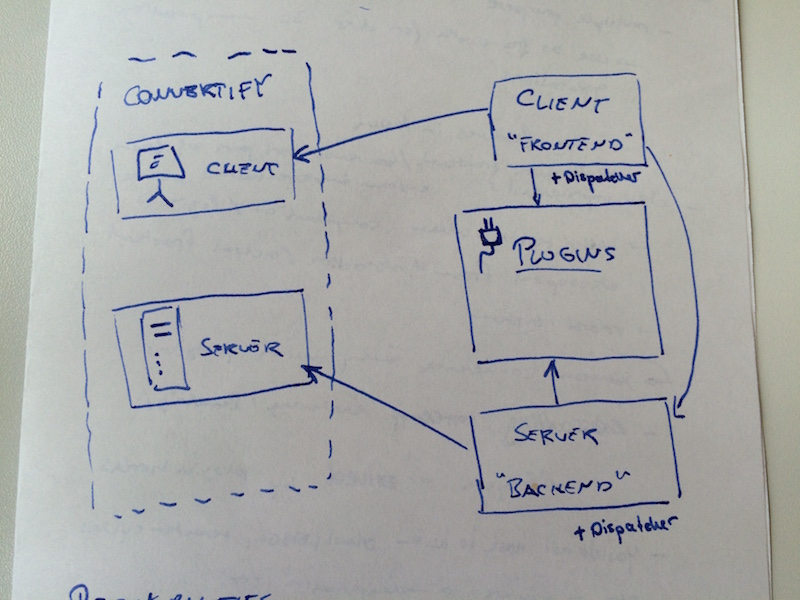
\includegraphics[width=1\columnwidth]{03-architecture_overview_current}
  \caption{Main Packages of the Platener Architecture}
  \label{fig:architectureOverviewCurrent}
\end{figure}

{\platener} is divided into the code packages {\convertify},
\name{Plugins} and \name{Client}.
Figure~\ref{fig:architectureOverviewCurrent} shows the
package diagram. Each package takes over a set of distinct
responsibilities.

\note{too generic here?}

The {\convertify} package is a framework, providing a
rendering engine and plugin management. The \name{Plugins}
package provides an exchangeable set of features for the
WebGL scene. The \name{Client} package gives the look and
feel of {\platener}. This package contains frontend
components, which make up the {\userinterface}. Also, a
\class{Dispatcher} is implemented in this package,
configuring the communication of plugins.

%     - needs-figure :: Client code connects all plugin
%     features with a user interface

%     - Use Framework to wire up everything, but not part of the
%       framework (Bundle and Protocols come in handy, Client code
%       implements a Dispatcher instance = the mediator)

%     - We have a WebApp and a Server package, which are both Client
%       code, because we have two types of applications
%     - the WebApp is an online service deployed for use by Makers
%     - the CLI tool is a service for batch processing or integration
%       with other applications

% **** The WebApp Package Builds a Cross-platform Web Page

%      - Subsubsection overview
%      - needs-ref :: Web Interfaces are built with HTML and CSS
%      - needs-ref :: The React library | copy from AOP paper
%      - needs-ref, needs-figure :: The Redux library (Dump Components and Smart Containers)
%      - needs-figure :: Using Redux dispatch in the Dispatcher
%      - Subsubsection summary

% **** The Server Package Allows Headless Batch Processing of Models

%      - Subsubsection overview
%      - A CLI tool runs in nodejs
%      - needs-ref :: Processing objects without opening a browser (isomorphic code)
%      - Processing multiple objects in sequence
%      - Integration with tools to be built in future
%      - Subsubsection summary


% \subsection{Package Responsibilities}

%  ensuring decoupled
% components. Thus a flexible, maintainable system is created.

% \emph{Convertify} provides generic tools which support plugins in manipulating
% {\threedmodel}s. This includes utilities for vector analysis as well as
% rendering routines and scene management. The application lifecycle can be
% initiated and observed via a \emph{Bundle}. A Bundle represents an instance of
% the application's computation unit. The Client and Server packages run a Bundle.

% \emph{Plugins} provide an exchangeable set of features which are used by the
% Client and Server package. A Plugin interacts with the Scene and its
% {\threedmodel}s via lifecycle events. E.g. a concrete conversion strategy
% provided by Platener is implemented by a single Plugin. Plugin features can be
% enabled for Client, Server or both.

% The \emph{Client} package gives the look and feel of the application. This
% package contains frontend components. The developer can choose any template
% engine\footnote{\url{http://www.sitepoint.com/overview-javascript-templating-engines/}}
% which serves the application's purpose. So the Client wires up the
% {\userinterface} and the computation logic.

% The \emph{Server} package is the headless\footnote{A headless web-application
%   runs without the graphical user interface of browsers.} counterpart to the
% Client package. A Command Line Interface enables the user to run the application
% without a browser. The Server also satisfies requests from the Client, such as
% caching and loading models in a RESTful
% interaction\footnote{\url{http://www.drdobbs.com/web-development/restful-web-services-a-tutorial/240169069}}.

% % \begin{itemize}
% % \item convertify: generic tools, helpers for 3d rendering, scene management,
% %   model manipulation, platener independent
% % \item client: look and feel, ux user interactions, wiring up/ firing up
% %   computations, implemented for platener
% % \item server: model storage/ cache, REST interaction, headless version of
% %   client, CLI-tool chain, implemented for platener
% % \item plugins: conversion specific computation and logic units, addons for
% %   frontend and backend, platener independent
% % \end{itemize}


% \subsection{Decoupling the Software into Packages}

% Decoupling the software into packages builds a robust system. Computation logic
% and UX components are kept apart, which allows isolated testing.

% \subsubsection{Dispatcher and Bundle on Client and Server}

% \myNotes{maybe put this up, so we understand earlier what the ClientDispatcher
%   is}

% The Server and Client package handle lifecycle events differently and use
% different protocols. That is because the Client package has to handle rendering
% and user interaction. The Server package merely computes the manipulated models
% and is used for batch processing of {\threedmodel}s. Therefore, we need two
% Dispatcher implementations for the client and for the server.

% A Bundle is the entry point for any client or server code. As the name
% indicates, a Bundle bundles all application code into a single instance. It
% references the specific \emph{ClientDispatcher} or \emph{ServerDispatcher},
% which are implemented in the Client or Server package respectively. Thus we can
% control the system by invoking protocol interfaces. The ClientBundle is exposed
% to the Client package. The ServerBundle is exposed to the ServerPackage.

% \section{Client Package}
% % ************************************************

% \subsection{Overview - Custom Frontend Code}

% \begin{itemize}
% \item when convertify framework, client is freespace to evolve yaself
% \item look and feel of the application
% \item task: connect logic to ui (speak with dispatcher) and build ui
% \item free choice of frontend framework (we take redux + react), but nothing
%   against jquery or angular or backbone or ...
% \item e.g. laser origami or brickify would choose a completely different
%   implementation of client -> custom per application
% \item react by facebook, redux by dan abramov, like flux architecure -> uni
%   directional dataflow, explicit state changes, data driven -> reduce side
%   effects and be efficient in coding and trace down errors easily
% \item \myNotes{diagram which shows benefits of flux architecture vs no flux
%     arch, look at intro vids for redux from dan abramov}
% \end{itemize}

% \subsection{React Templates}

% \begin{itemize}
% \item show html tree graph and how data communication goes wild when talking
%   with siblings
% \item ideally dumb components (dont know where data is coming from, just display
%   it)
% \item stateless, components directory
% \item WIP: before no redux, so there are some mixed up components left :S
% \item show short example how a dump component looks like, \myNotes{listing!}
% \end{itemize}

% \subsection{Redux Data-driven Control Flow}

% \begin{enumerate}
% \item Redux `dispatch` and state
%   \begin{itemize}
%   \item one state container
%   \item functional, no side effects
%   \item maybe copy or reference redux description (just explain why its awesome)
%   \item injected into react via context
%   \end{itemize}

% \item Smart Containers
%   \begin{itemize}
%   \item connect to state
%   \item containers know where data is from (vs dump components)
%   \item fitler and preprocess raw data, setup interaction events to trigger
%     actions
%   \item give data and callbacks to a component (they setup the actual ui, but
%     contain no visible elements themselves)
%   \item \myNotes{listing show how to connect and use component from other
%       listing}
%   \end{itemize}

% \item Manage Async Plugin Hell
%   \begin{itemize}
%   \item as described before, plugin data is not available on load
%   \item we can use Dispatcher and redux dispatch combined
%   \item protocols -> state change in plugins -> dispatch -> state change in
%     frontend
%   \item no polling or observing of data, fully reactive (system -> client communication)
%   \item as client has access to bundle, we can call interfaces exposed by
%     protocols (client -> system communication)
%   \end{itemize}
% \end{enumerate}

% \section{Server Package}
% % ************************************************

% \subsection{Overview - Custom Server Code}

% \begin{itemize}
% \item like client, can have custom implementations
% \item we have caching and cli (headless version of application)
% \item requires isomorphic code: execute on client and server equally
% \item \myNotes{isomorphic means...}
% \item threejs, polyfills, \myNotes{...}
% \end{itemize}

% \subsection{Model Cache}

% \begin{itemize}
% \item idea: build up repository of models when users interact with it
% \item taken from brickify: uploading meshlib version of model
% \end{itemize}

% \subsection{Test Pipeline}

% \begin{enumerate}
% \item WHY do we have a Test Pipeline?
%   \begin{itemize}
%   \item robustness tests
%   \item batch processing
%   \item headless version for integration with other projects
%   \item failure detection because of diversity of objects
%   \end{itemize}

% \item Headless Conversion of Objects
%   \begin{itemize}
%   \item run solutionselection plugin also
%   \item but dispatcher is setup a bit differently
%   \item no recomputation, no grid, no visualizer
%   \item scene manager will not render anything (unless, WIP we exchange webgl
%     rendering with headlessgl to produce screenshots of each conversion)
%   \item cli tool -> safe results into directories
%   \end{itemize}

% \item Reports
%   \begin{itemize}
%   \item = extended console logs
%   \item show how conversion was going
%   \item display failures, status, progress
%   \item in the end: sum up + give stats
%   \item WIP: current problems: not all conversions are garbage collected
%     correctly, will run out of memory after some conversions -.- (maybe nobody
%     has to know about that)
%   \end{itemize}

% \item Benchmarks
%   \begin{itemize}
%   \item xxx testmodels
%   \item we proposed mostly stacked as the best solution
%   \item too many arbitrary forms hindered plate conversion
%   \item just shows conversion stats (maybe all models vs box category only)
%   \item \myNotes{measure times for conversions and evaluate}
%   \end{itemize}
% \end{enumerate}

\iffalse


\section{Architecture Overview}
% ************************************************

\begin{figure}
  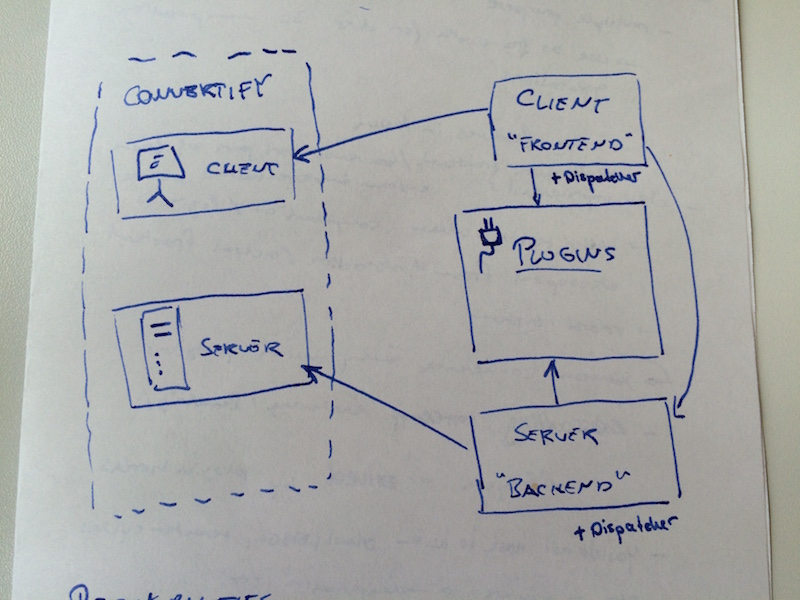
\includegraphics[width=1\columnwidth]{03-architecture_overview_current}
  \caption{Main Packages of the Platener Architecture}
  \label{fig:architectureOverviewCurrent}
\end{figure}

Platener is designed to enable web-based manipulation and rendering of
{\threedmodel}s. Figure \ref{fig:architectureOverviewCurrent} shows the major
packages \emph{Convertify}, \emph{Client}, \emph{Server} and \emph{Plugins}. The
arrows indicate dependencies between the packages. The architecture emphasizes a
uni-directional data and event flow. Similar to mobile application design,
lifecycle events and the concept of
delegation\footnote{\url{https://developer.apple.com/library/ios/documentation/General/Conceptual/DevPedia-CocoaCore/Delegation.html}}
establish clear communication among packages.

% \begin{itemize}
% \item platener built on top of...
% \item 4 major packages: convertify, client, server and plugins
% \item optimized towards: working with 3d-models in webgl environment
% \item plugin-based: allow interchangeable computation logic/ conversion methods
% \item combination of lifecycle-based communication and explicit calls via
%   dispatchers (related work: mobile application design, mediator pattern) \ritem
%   explicit communication between packages
% \end{itemize}

\subsection{Package Responsibilities}

Each package takes over a set of distinct responsibilities ensuring decoupled
components. Thus a flexible, maintainable system is created.

\emph{Convertify} provides generic tools which support plugins in manipulating
{\threedmodel}s. This includes utilities for vector analysis as well as
rendering routines and scene management. The application lifecycle can be
initiated and observed via a \emph{Bundle}. A Bundle represents an instance of
the application's computation unit. The Client and Server packages run a Bundle.

\emph{Plugins} provide an exchangeable set of features which are used by the
Client and Server package. A Plugin interacts with the Scene and its
{\threedmodel}s via lifecycle events. E.g. a concrete conversion strategy
provided by Platener is implemented by a single Plugin. Plugin features can be
enabled for Client, Server or both.

The \emph{Client} package gives the look and feel of the application. This
package contains frontend components. The developer can choose any template
engine\footnote{\url{http://www.sitepoint.com/overview-javascript-templating-engines/}}
which serves the application's purpose. So the Client wires up the
{\userinterface} and the computation logic.

The \emph{Server} package is the headless\footnote{A headless web-application
  runs without the graphical user interface of browsers.} counterpart to the
Client package. A Command Line Interface enables the user to run the application
without a browser. The Server also satisfies requests from the Client, such as
caching and loading models in a RESTful
interaction\footnote{\url{http://www.drdobbs.com/web-development/restful-web-services-a-tutorial/240169069}}.

% \begin{itemize}
% \item convertify: generic tools, helpers for 3d rendering, scene management,
%   model manipulation, platener independent
% \item client: look and feel, ux user interactions, wiring up/ firing up
%   computations, implemented for platener
% \item server: model storage/ cache, REST interaction, headless version of
%   client, CLI-tool chain, implemented for platener
% \item plugins: conversion specific computation and logic units, addons for
%   frontend and backend, platener independent
% \end{itemize}


\subsection{Decoupling the Software into Packages}

Decoupling the software into packages builds a robust system. Computation logic
and UX components are kept apart, which allows isolated testing.

\subsubsection{Convertify Is a Framework}

The \emph{Convertify} package is meant to be used as a white-box framework for building
3D manipulation applications. Platener is such an application, supporting model
imports, rendering, altering and export of geometries. Introducing a web
framework makes sense, because WebGL gets more and more stable as of the year
2016 \myNotes{TODO: reference!}. Thus graphics software can be brought to huge
audience providing cross-platform web services. For example \emph{Brickify} or \emph{Laser
Origami}\myNotes{ref} could be implemented with \emph{Convertify}.

% \begin{itemize}
% \item multpiple purpose:
% \item use as (whitebox) framework for other 3D manipulation applications (related work:
%   mechanism mining, etc)
% \item web service --> highly available, cross platform
% \item plug features in and out
% \item because concrete frontend/ backend not part of framework, custom
%   implementations possible (no vendor lock) \myNotes{this should be part of the
%     comparison with Brickify}
% \end{itemize}

\subsubsection{Plugins Establish Focus on Graphic Problems}

Plugins are self-contained units which mainly interact with the WebGL scene and
its scene graph. Whole feature-sets can be switched on or off at once. They are
loosely coupled but have high cohesion at the same time. This prevents spaghetti
code and supports maintainability of each component. Furthermore, we use
software hooks to integrate plugins with rendering of models and access to
geometry data. This event-based approach enables developers to write a 3D
manipulation tool without having detailed domain knowledge about WebGL and
web-services. This allows developers from the Computer Graphics domain to
concentrate on the graphics problem, rather than the web-environment.

% \begin{itemize}
% \item dev improvements:
% \item better testing of computation/ logic because decoupled from ux
% \item robust system
% \item --> loose coupling of plugins, high cohesion in plugins
% \item --> isolated testing/ development possible
% \item solve cross-cuts: rendering/ loading <> lifecycle of plugins (eventbased)
% \item you do not have to know about WEBGL, render cycles etc. to provide a 3D
%   manipulation tool
% \item --> minimize web-domain knowledge as CG-devs are often unfamiliar with
%   this environment
% \end{itemize}

% \subsection{Discussion "vs Brickify"}

\subsubsection{A Comparison with the Brickify Packages}
\myNotes{maybe put statement, rather then description into headline}

The Convertify package is not present in the Brickify architecture, see Figure
\ref{fig:architecture_overview_brickify}. This means Brickify provides a mix of
UX components, computation logic and interfacing code in the Client and Server
packages. Plugin communication is hard to observe and only implicitly ordered.
We introduce the new package to escape the vendor lock\myNotes{explain vendor
  lock} of previously used UX libraries. Libraries like \myNotes{add refs}
\emph{jQuery} and \emph{Jade} \myNotes{now pug} scatter code throughout the
project. By removing UX dependencies from logic components we create a
thoroughly testable code base.

\begin{figure}
  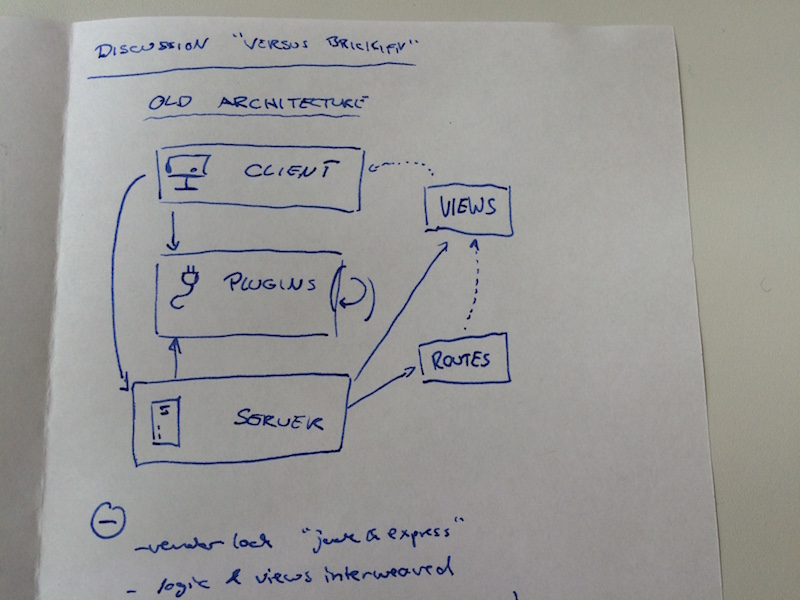
\includegraphics[width=1\columnwidth]{03-architecture_overview_brickify}
  \caption{Main Packages of the former Brickify Architecture}
  \label{fig:architecture_overview_brickify}
\end{figure}

% \textbf{pros}
% \begin{itemize}
% \item fast enhancements as only views/ routes have to be adapted
% \item less interfacing because frontend <> logic tightly coupled
% \end{itemize}
% \textbf{cons}
% \begin{itemize}
% \item vendor lock: jade and express
% \item logic and views interweaved: high coupling --> hard testing, hard
%   maintainability, hard to change things
% \item implicit plugin communication
% \item complex management of custom 3d manipulation tools would require a lot of
%   rewrites because of view/ logic mix
% \end{itemize}

\section{Convertify Package and its Plugin Architecture}
% ************************************************

Platener uses the Convertify package as entry points to the {\threedmodel}
processing. The package provides features for browser- and
headless-environments.

It encapsulates basic logic for {\threedmodel} manipulation and model import.
Additionally, we provide utilities to simplify working with \emph{\threejs} or
rendering objects into scene.

Convertify handles the scenegraph of the application. \emph{Nodes} are injected
into the scene \myNotes{ref brickify} and lifecycle events are emitted, e.g. on
load, on draw or on touch interactions with the \emph{Node}.

% \begin{itemize}
% \item entry points
% \item headless startup
% \item basic logic for 3dmodel manipulation (import, mesh-conversion)
% \item scenegraph and rendering (nodes, refs for sync objects in Brickify)
% \item plugin interaction (hooks)
% \item application helpers (threeHelper, renderHelper, commons (we should move
%   commons to convertify))
% \end{itemize}

\subsection{Scene Graph and Scene Management}

\myNotes{this is crap somehow}
The scene graph is built from \emph{Nodes}. Each \emph{Node} is associated
with a single \emph{THREE.Object3D} instance. This instance is rendered by the
WebGL renderer. The \emph{Node} is a high-level abstraction of objects in the
scene graph. \emph{THREE.Object3D} instances contain fine-grained sub-objects and
actual vertices. For each Plugin we provide further \emph{THREE.Object3D}
instances, which belong to the \emph{Node}'s \emph{THREE.Object3D}.

\emph{Nodes} belong to a \emph{Scene}. Multiple \emph{Scenes}
are added to a \emph{Project}. The \emph{Project} is the single root node of the
scene graph. \emph{Nodes} are added and removed by the \emph{SceneManager},
which is controlled in a \emph{Bundle}.

% For each \emph{Plugin} we provide further \emph{THREE.Object3D}
% instances, to which the \emph{Plugins} can append their computed visuals.

% \begin{itemize}
% \item project -> scene (one active, multiple hidden) -> node
% \item a single project per application
% \item manages a scene (shallow representation of actual WEBGL scene, high level
%   objects)
% \item node - object in the scene (represents arbitrary data loaded into scene,
%   has transforms)
% \item the model you see is a node
% \item rendering in Renderer (WebGL renderer abstraction)
% \item update loop, plugins may manipulate the model -> changes displayed
% \end{itemize}

\subsection{Lifecycle Events with Plugin Hooks}

\subsubsection{The Internal System Emits Lifecycle Events}

Similar to other applications\myNotes{what applications?}
\emph{Convertify} dispatches events from the internal system during
the application's lifecycle. The internal system refers to framework
features, which all applications built with \emph{Convertify} share.
Such features are model import, scenegraph manipulation or render
updates.

\myNotes{add figure environment here}

The lifecycle of \emph{Convertify} is depicted in Figure \myNotes{add
  figure for platener lifecycle}. First we initialize all activated
plugins in the \emph{init} event. During the \emph{init3d} event each
plugin is passed an empty \emph{THREE.Object3D} instance. We call it
the root node. The root node is associated with the \emph{Node} in the
scene graph. The plugins append the computed visuals onto the root
node. All root nodes are rendered by the \emph{Renderer}, calling the
\emph{update3d} callback. \myNotes{look up event name}. When a
\emph{Node} from the \emph{Scene} is selected by the user, we dispatch
the \emph{onNodeSelect} event. When a new \emph{Node} is added to the
\emph{Scene}, the \emph{onNodeAdd} hook is triggered. The
\emph{onNodeRemove} hook is triggered respectively when a \emph{Node}
is removed from the \emph{Scene}. \myNotes{ref brickify}

% \begin{itemize}
% \item plugin init - plugin is loaded, general setup
% \item scene init -
% \item scene adding
% \item scene rendering/ update/ brushing
% \item scene selecting
% \item scene removing
% \end{itemize}

% \begin{itemize}
% \item App Lifecycle: Model Loading
% \item Plugin Init
% \item Scene Refreshes
% \item Scene Graph Interactions
% \item refer to Brickify
% \end{itemize}

\subsubsection{Plugins Interact with the Internal System via
  Lifecycle Events}

The subscribers to lifecycle events are \emph{Plugins}. Each event
type exposes a \emph{PluginHook}. Each \emph{Plugin} registers a
callback on an arbitrary number of events. These callbacks get
called when the event is dispatched by the system. Thus plugins can
handle each event and apply their own functionality to the scene or
even the model geometry. With this we emphasize compact computation
units in plugins, which can still interact freely with the system.
The approach is directly adapted from \emph{Brickify} \myNotes{ref
  chapter in brickify}.

% \begin{itemize}
% \item Gain control for computation units (plugins)
% \item interact with the system
% \item plugin hooks (refer to pluginHooks.yaml)
% \item called on each plugin
% \item allow plugin to handle the event (e.g do some manipulation to the scene)
% \end{itemize}

\subsection{Plugins within Convertify}

A \emph{Plugin} bundles methods and system event callbacks to
provide a new set of features to the application, e.g. the
\emph{PlatenerPipeline} plugin builds a two-dimensional construction
plan from the {\threedmodel} and exposes it for download. The
\emph{Plugin} can be switched on or off on application load for the
Client and Server package respectively. Complex applications can be
built by composing multiple plugins. This supports the framework
character of applications built with Convertify.


% \begin{itemize}
% \item part of the Plugin Package
% \item pluggable set of feature
% \item or self-contained unit
% \item can be activated for server/ client
% \item composing multiple plugins --> extensible, maintainable method of building
%   complex applications
% \end{itemize}


% \begin{itemize}
% \item Convertify as a framework
% \item do not mix logic/ ui
% \item decomposable logic (no spaghetti code)
% \end{itemize}


\subsubsection{Plugins Are Packages of Their Own}

Each \emph{Plugin} resides in the Plugin Package. We define a
\emph{package.json} file, which contains metadata of the package, see Listing
\ref{lst:packagejson}. Conceptionally, a \emph{Plugin} can be a separate
\emph{npm} package\footnote{Node Package Manager,
  \url{https://docs.npmjs.com/getting-started/what-is-npm}}. This means plugins
could be installed like any other typical dependency. For the sake of
development speed, we do not use the \emph{npm} setup yet. \myNotes{ref brickify}

\begin{listing}[ht]
\begin{minted}[
linenos
]{json}
{
  "name": "platener-pipeline",
  "version": "1.0.0",
  "description": "modifies model mesh to enable lasercuttable parts",
  "browser": "./PlatenerPipeline.coffee",
  "main": "./PlatenerPipeline.coffee"
}
\end{minted}
\caption{\emph{package.json} file of \emph{PlatenerPipeline} plugin.}
\label{lst:packagejson}
\end{listing}

To register a \emph{Plugin} with \emph{Convertify}, we have to add an entry in
the \emph{PluginMap}. The \emph{PluginMap} is a static dictionary, enumerating
all installed plugins and their filepaths. Because \emph{\nodejs} as well as
\emph{\essix} do not support dynamic require statements\footnote{A dynamic
  require statement can include and interpret source files into runtime where
  file paths are generated during runtime.}, we have to list each package
explicitly. In future systems we could alter the build system to include plugin
files automatically before compilation step.

The exposed main file of the package implements a set of \emph{PluginHooks}.
These hooks are registered at the \emph{Dispatcher}, which is responsible for
dispatching the lifecycle events to the plugins in a predefined order\myNotes{,
  see chapter ??}. Beside \emph{PluginHooks}, a \emph{Plugin} can expose
\emph{Protocols} to interact with the system. \emph{Protocols} are described in
\myNotes{chapter ??}. A plugin implements any internal structure or
complexity. The simplest form of a plugin is a single file. But it may provide a
whole filetree. A list of plugins used in \emph{Platener} is describe in
\myNotes{chapter ??}.


% \begin{itemize}
% \item define with package.json (could conceptionally be another npm package) =
%   metadata
% \item add to PluginMap
% \item define hooks
% \item invoked by Dispatcher
% \item space of freedom is huge...
% \item make this very concrete, to show how to write your own plugins
% \end{itemize}

% \myNotes{see chapter ??, a list of plugins}
% \myNotes{see chapters ?? for more detail (nodevis, platenerpipeline, ...)}
% \myNotes{look into control flow to understand plugin invokations}
% \myNotes{maybe figure about lifecycle and hooks}


\subsection{Control Flow and Plugin Communication}

As Platener is composed of multiple plugins, which either represent
computation logic or render components, we have to know exactly when
each of these plugins will interact with the system. We propose a
Dispatcher component, behaving similar to the mediator
pattern\footnote{\url{https://sourcemaking.com/design_patterns/mediator}}.

\subsubsection{The Dispatcher is a Mediator}

The Dispatcher loads and initializes a set of configured plugins. It organizes
the communication between plugins and client, plugins and server and plugins and
plugins in a single place, as shown in
Figure~\ref{fig:architecture_overview_dispatcher}. The \emph{PluginLoader}
instantiates each plugin and exposes all defined \emph{PluginHooks} to the
\emph{Dispatcher}. \myNotes{this is all similar to brickify, ref please}

% \begin{itemize}
%   \item dispatcher is entry point for client -> logic, server -> logic
%   application
% \item loads and init given list of plugins via pluginloader
% \item implements each plugin hook and decides how to dispatch each call to the
%   plugins dependent on application state
% \end{itemize}


Convertify fires lifecycle events on which the plugins can react. The mediator
knows an explicit execution order for each plugin when a lifecycle event is
fired. Figure~\ref{fig:architecture_dispatcher_pipeline} shows in detail how the
\emph{PlatenerPipeline} plugin and the \emph{Dispatcher} communicate via events.
Codewise, the \emph{Dispatcher} implements each plugin hook and remits the event
to the loaded plugins.

\begin{listing}[!h]
\centering
\begin{minted}[
linenos
]{coffeescript}
class ClientDispatcher extends AbstractDispatcher

  #
  # ...
  #

  hooks:
    init: (bundle) ->
      return @callAllPlugins('init', bundle)

    onNodeAdd: (node) ->
      return [
        @callPlugin('solution-selection', 'onNodeAdd', node),
        @callPlugin('node-visualizer', 'onNodeAdd', node)
      ]

    onNodeRemove: (node) ->
      return [
        @callPlugin('node-visualizer', 'onNodeRemove', node)
        @callPlugin('solution-selection', 'onNodeRemove', node)
      ]
}
\end{minted}
\caption{The \emph{ClientDispatcher} implements plugin hooks to remit lifecycle events.}
\label{lst:client-disp-hooks}
\end{listing}

Listing \ref{lst:client-disp-hooks} shows, how the
\emph{ClientDispatcher} \myNotes{client dispatcher explained??}
handles the \textit{init}, \textit{onNodeAdd} and
\textit{onNodeRemove} hooks. By remitting events manually, we have
fine-grained control about the execution order. This is necessary,
because we want to invoke the \emph{PlatenerPipeline} plugin,
computing the construction plans, before rendering the results via
the \emph{NodeVisualizer} plugin. Also we have to remove the
\emph{NodeVisualizer} results before deleting the data, to avoid
reference errors. For both \emph{PluginHooks} the plugins are
executed in a different ordering.

% \begin{itemize}
% \item refer to Brickify, PluginLoader
% \item explain plugins.yaml shortly
% \item implements plugin hooks itself (show code snippets, hooks property)
% \end{itemize}

\begin{figure}
\centering
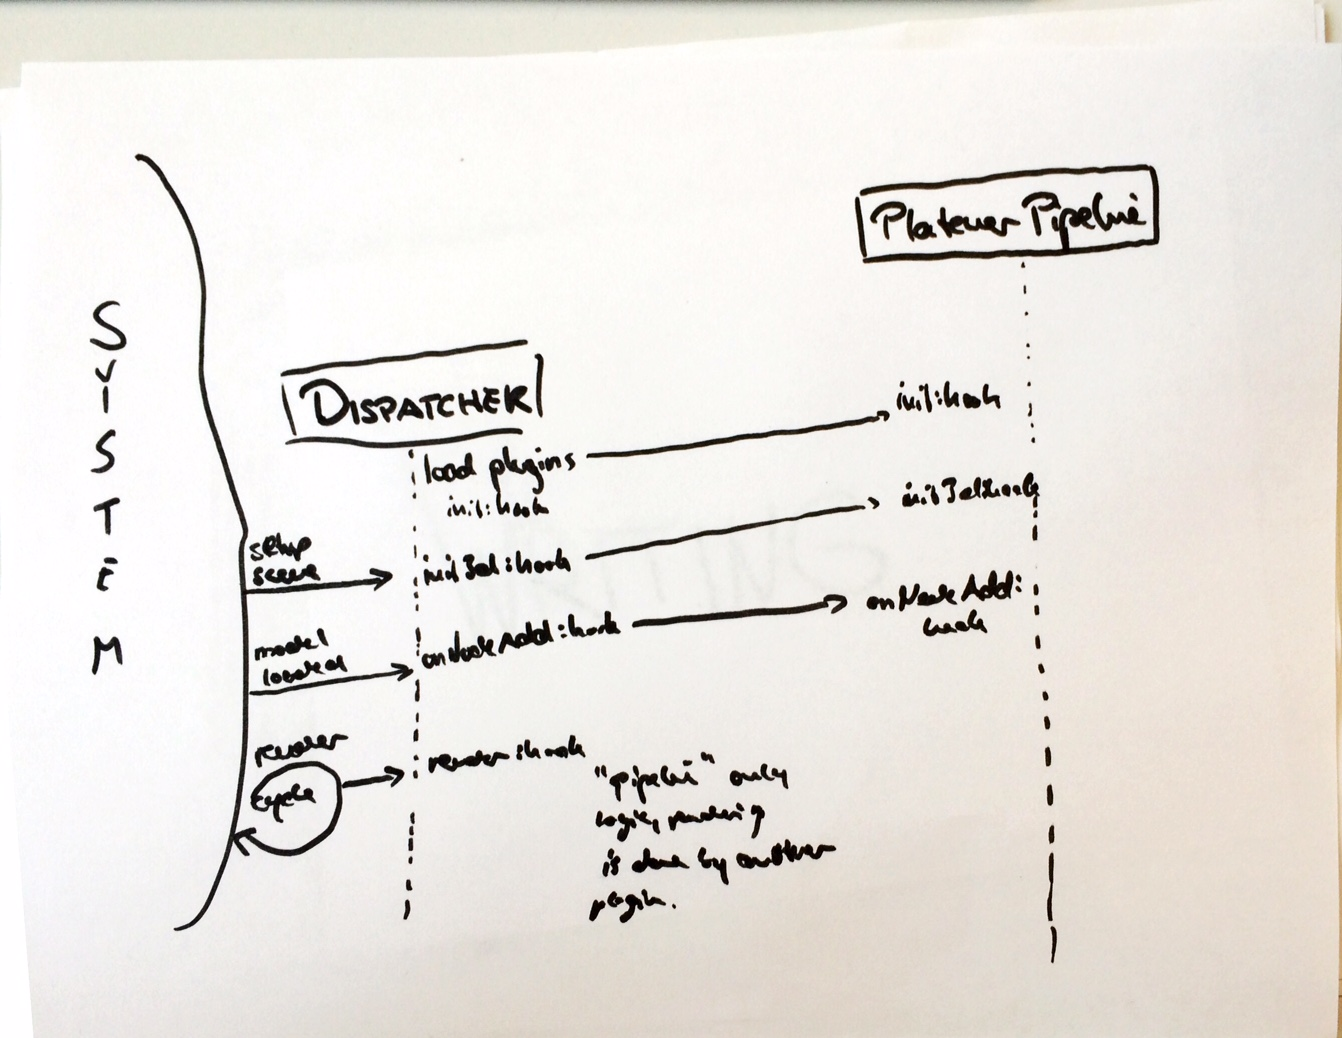
\includegraphics[width=1\columnwidth]{03-architecture_dispatcher_pipeline}
\caption{Dispatcher and PlatenerPipeline communicate via lifecycle events.}
\label{fig:architecture_dispatcher_pipeline}
\end{figure}

To allow communication between plugins themselves or plugins and
Client, we use \emph{Protocols} because \emph{PluginHooks} are not
flexible enough. A \emph{Protocol} defines an interface, which has
to be implemented by a \textit{delegate}. Via
delegation\footnote{\url{http://best-practice-software-engineering.ifs.tuwien.ac.at/patterns/delegation.html}}
we define callbacks which are invoked by Plugins on the Dispatcher.
The Dispatcher then notifies server, client or other plugins.
Furthermore, \emph{Protocols} can add a set of methods to the
Dispatcher via meta programming.

Listing \ref{lst:solutionselectiondelegate} shows the definition of
the SolutionSelectionDelegate protocol. It requires its implementing
class to provide the methods \textit{evaluationDidStart},
\textit{evalutionOfMethodDidFinish}, \textit{evaluationDidFinish},
\textit{evaluationDidFail} and
\textit{evaluationDidFailWithSolutions}. Listing
\ref{lst:client_dispatcher_protocol} shows the
\emph{ClientDispatcher} implementing the
\textit{evaluationDidFinish} method. By providing the callbacks, the
Dispatcher knows about the current state of the conversion and its
completion. For example, we render all solutions after their
computation. To satisfy the SolutionSelectionDelegate protocol, the
Dispatcher also implements the remaining methods.

\begin{listing}[!h]
\centering
\begin{minted}[
linenos
]{coffeescript}
SolutionSelectionDelegate = {
  shouldImplement: [
    # Invoked before a method is evaluated.
    'evaluationDidStart'
    # Invoked after each method finished.
    'evaluationOfMethodDidFinish'
    # Invoked after all methods finished.
    'evaluationDidFinish'
    # Invoked when an error occured in solution selection.
    'evaluationDidFail'
    # Invoked when errors occur in pipeline steps during computation
    'evaluationDidFailWithSolutions'
  ]
}
\end{minted}
\caption{\emph{SolutionSelectionDelegate} protocol definition}
\label{lst:solutionselectiondelegate}
\end{listing}

\begin{listing}[!h]
\begin{minted}[
linenos
]{coffeescript}
class Dispatcher extends AbstractDispatcher
  ### Solution Selection ###
  @protocol(SolutionSelectionDelegate)

  #
  # ... more protocol methods ...
  #

  evaluationDidFinish: (solutions) ->
    @getPlugin('node-visualizer').render(solutions)
\end{minted}
\caption{\emph{ClientDispatcher} implements the \emph{SolutionSelectionDelegate}
  protocol}
\label{lst:client_dispatcher_protocol}
\end{listing}

% https://developer.apple.com/library/ios/documentation/General/Conceptual/DevPedia-CocoaCore/Delegation.html
% \textbf{protocols}
% \begin{itemize}
% \item communication between packages (no lifecycle)
% \item use protocols (explicit definition of what will happen)
% \item protocol embodies a set of feature for the application
% \end{itemize}


\subsubsection{The Dispatcher is the Single Source of Truth}
\label{sec:disp-single-source}

When applications grow, it is hard to observe all messaging between
components at once. With the \emph{Dispatcher}, we control all
communication between the packages at one place. Without implicit
ordering of callback executions, we can trace erroneous behavior
fast. The design of a singleton controlling the application's
lifecycle is known from frameworks in mobile application
development, like Android\ref{??} or iOS\ref{??}.

The usage of \emph{Protocols} helps developers keep track of
interfaces between components. We enforce this concept, because
\javascript is a dynamically typed programming language. Statically
typed programming languages pay out, when projects grow large.
Unexpected type and interface errors happen less often. Because of
the web-environment and previous work, we are bound to
\coffeescript. Thus, we emphasize explicit structuring of interfaces
via \emph{Protocols}.

% \begin{itemize}
% \item one guy who pulls all the strings (one source of truth)
% \item look up all communications between decoupled components here
% \item similar designs in known application frameworks (android, ios)
% \item javascript, non-type language --> protocols ensure correct interfaces
% \end{itemize}

%\begin{itemize}
% \item implements protocols for plugins (show code snippets)
% \item explain how plugins push state (control-flow information) back to the
%   dispatcher
%\end{itemize}

\begin{figure}
  \centering
  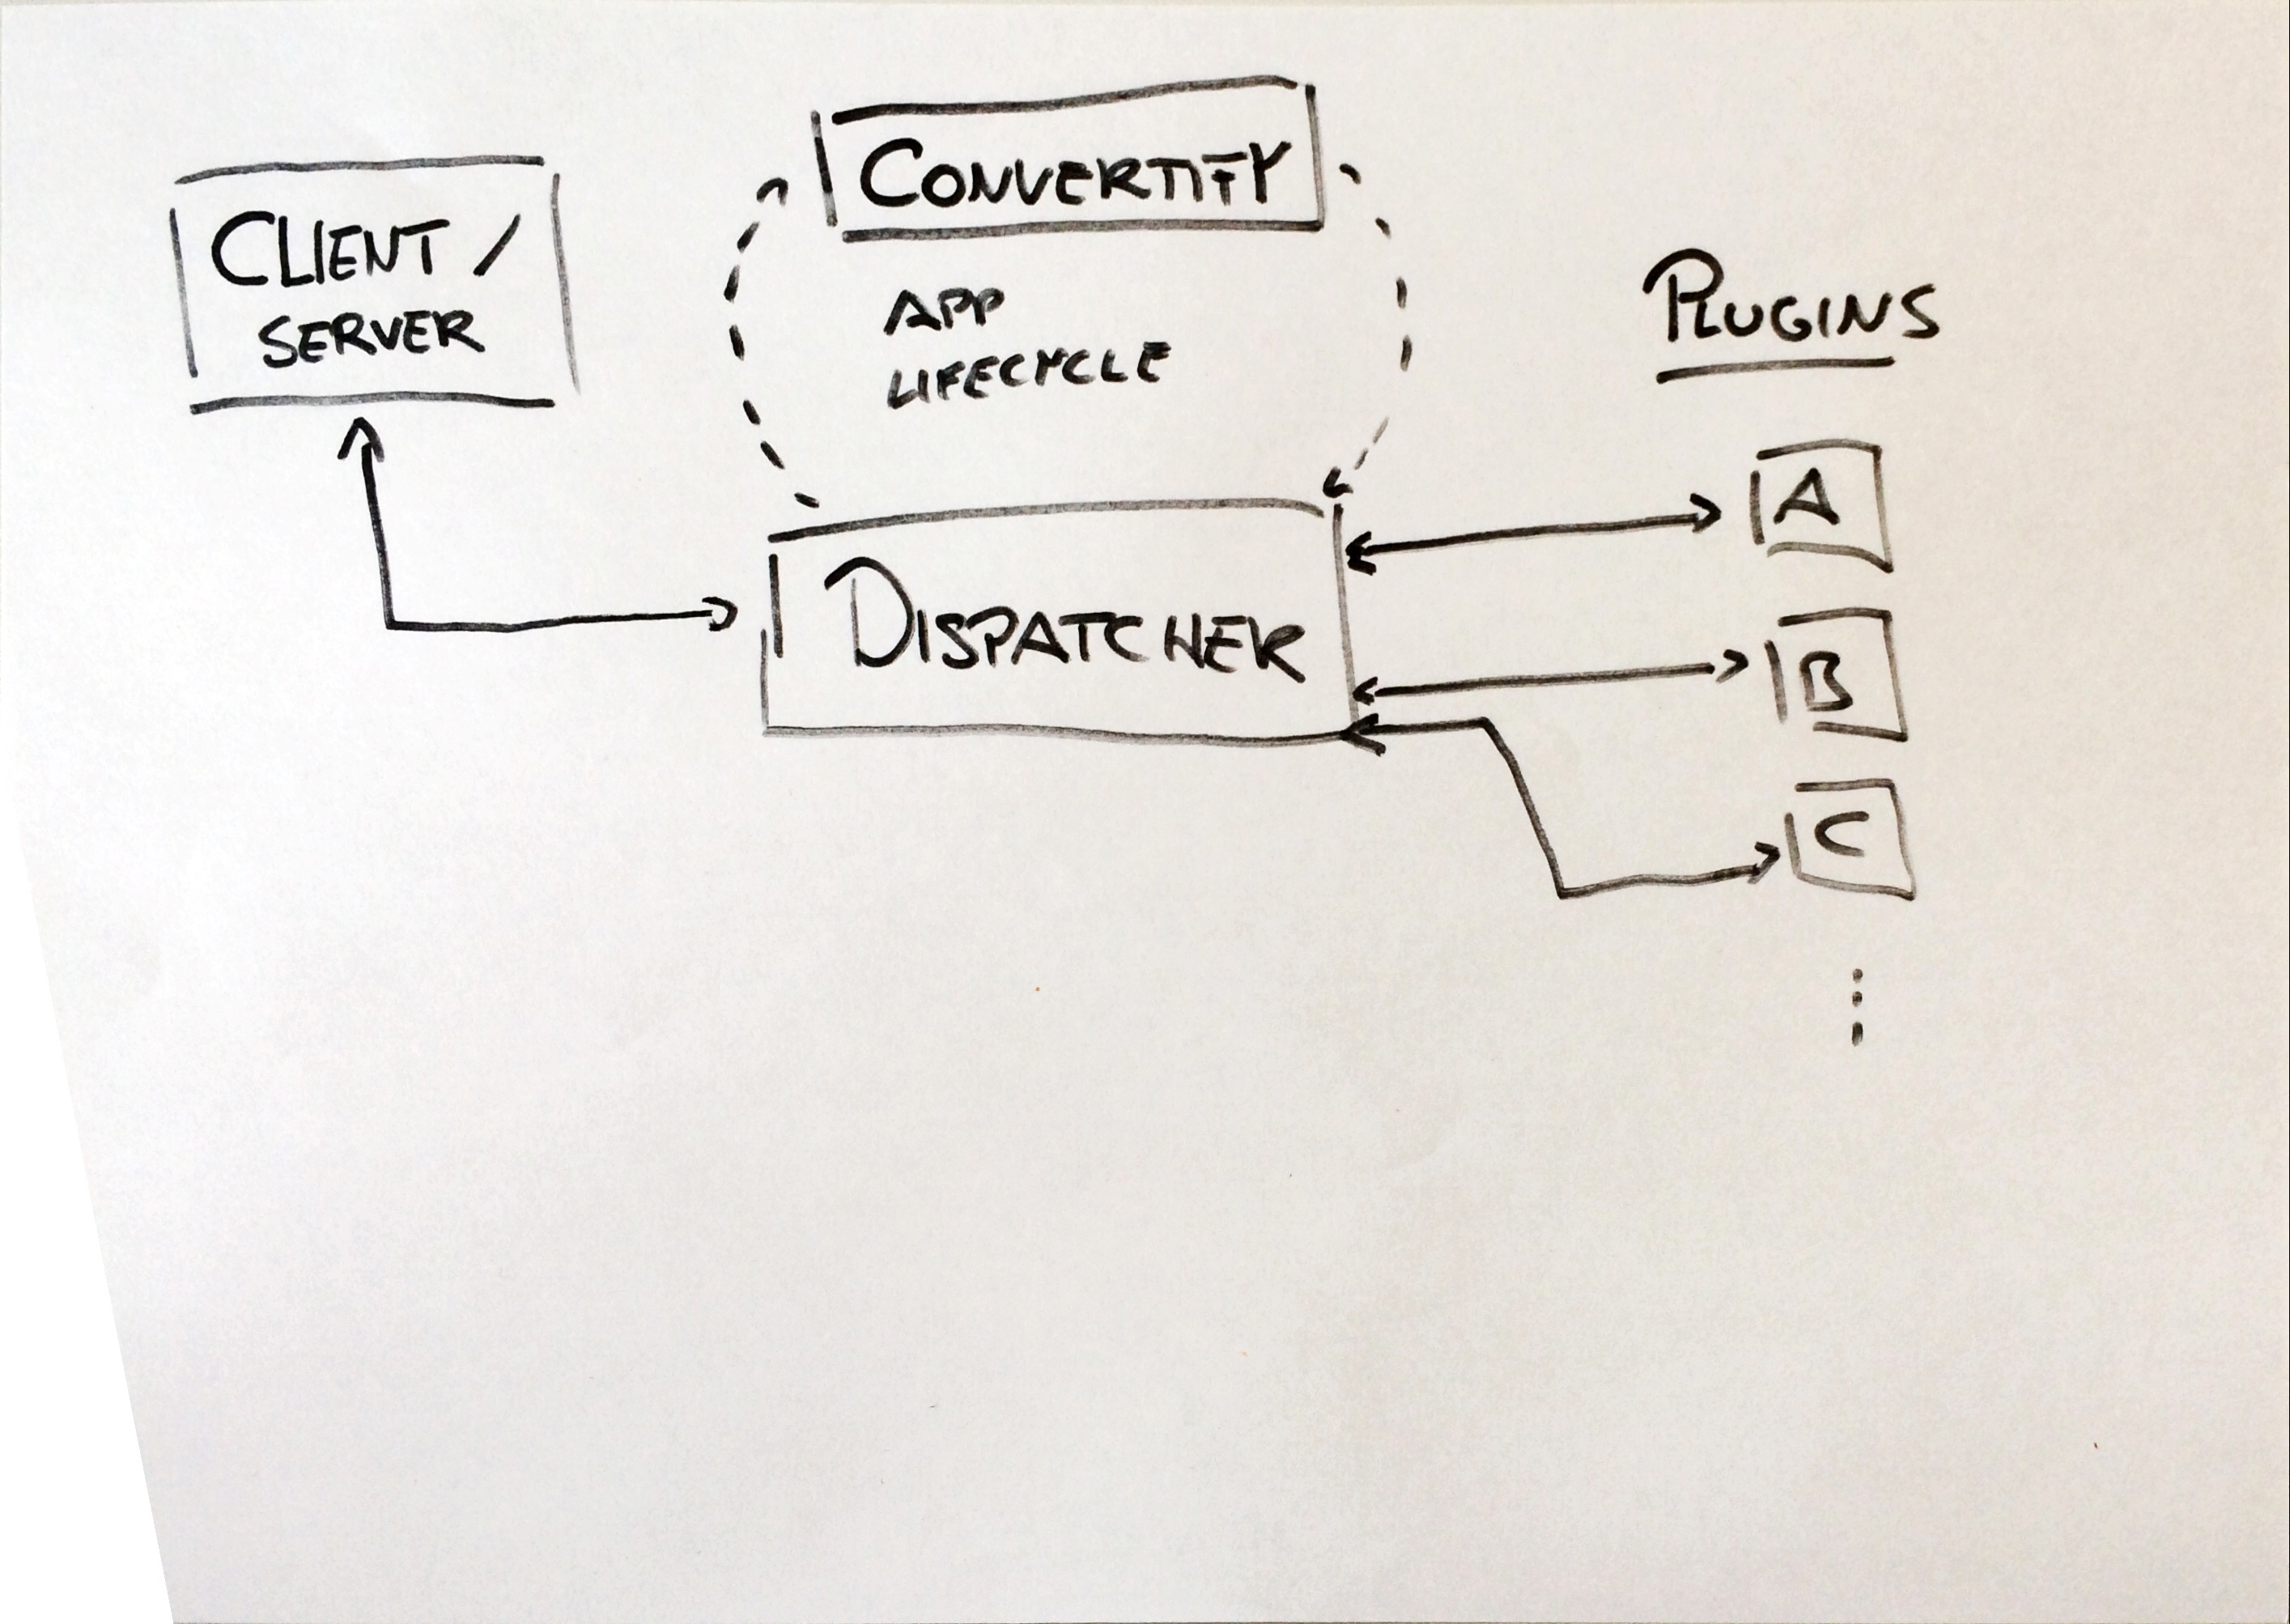
\includegraphics[width=1\columnwidth]{03-architecture_overview_dispatcher}
  \caption{Dispatcher manages inter-application communication during the
    lifecycle of the app.}
  \label{fig:architecture_overview_dispatcher}
\end{figure}

\subsubsection{Dispatcher and Bundle on Client and Server}

\myNotes{maybe put this up, so we understand earlier what the ClientDispatcher
  is}

The Server and Client package handle lifecycle events differently and use
different protocols. That is because the Client package has to handle rendering
and user interaction. The Server package merely computes the manipulated models
and is used for batch processing of {\threedmodel}s. Therefore, we need two
Dispatcher implementations for the client and for the server.

A Bundle is the entry point for any client or server code. As the name
indicates, a Bundle bundles all application code into a single instance. It
references the specific \emph{ClientDispatcher} or \emph{ServerDispatcher},
which are implemented in the Client or Server package respectively. Thus we can
control the system by invoking protocol interfaces. The ClientBundle is exposed
to the Client package. The ServerBundle is exposed to the ServerPackage.

\subsubsection{Brickify uses PluginHooks only}

\emph{Brickify} dispatches plugin hooks directly from the internal system to the
plugins without using a mediator in between. Compared to \emph{Convertify}, it
does not require any boilerplate code to setup the communication.
\emph{Convertify} needs a custom integration of each \emph{Plugin} into its
\emph{Disptacher}.

On the other hand, \emph{Brickify} could not control the ordering of
\emph{PluginHook} invokations. It is implicitly defined by the loading sequence
of plugins. Furthermore, the frontend code needs to access plugin data. The data
is only available after the plugins are loaded or even specific hooks were
executed. Via a mediator we can notify the frontend about state changes, rather
than asyncronically trying to poll the data.

With the introduction of a \emph{Dispatcher}, \emph{Plugins} now can push state
back to the system and implement \emph{Protocols} for more control over the
communication.

% \begin{itemize}
% \item wiring up plugins
% \item explicitly calling plugin hooks
% \item highly customizable when adding in new plugins
% \item how is control flow achieved? -->
% \end{itemize}

% \begin{itemize}
% \item ++ pros
% \item loading sequence control (impossible to repair)
% \item fine grained scheduling of communication
% \item explicit execution behavior
% \item ... (look at notes on desk)
% \item
% \item -- cons
% \item boilerplate code
% \item custom integration for each plugin
% \end{itemize}

% \begin{itemize}
% \item ++ pros
% \item no further config needed
% \item
% \item -- cons
% \item implicit order
% \item in different use cases, different plugins have to interact first (order is
%   not fixed)
% \item frontend often has to work on data which is not available before another
%   plugin loaded
% \end{itemize}

% \myNotes{now plugins can...}

% \begin{itemize}
% \item push application state back to the dispatcher
% \item communication with each other by specifying a protocol which has to be
%   implemented on the mediator
% \item mediator then can oversee the communication
% \end{itemize}

\section{Plugins in Platener}
% ************************************************

\subsection{Plugin Overview}

% The Client package provides the look and feel of Platener. The Server package
% manages communication between frontend and data storage.

The plugins composed into Platener provides its computation logic and WebgGL
scene rendering. We will give a brief introduction of each plugin in the
following paragraphs.

\subsubsection{Coordinate System}

This plugin provides orientation enhancements for the WebGL scene. Rendering
xyz-axes and a an axis-aligned grid, users can grasp alignment and dimensions of
{\threedmodel}s. Figure \ref{fig:architecture_overview_coordinate_system} shows
the coordinate system in the WebGL view. The Coordinate System is taken from
\emph{Brickify} as is\footnote{ref original code file}.

\begin{figure}
  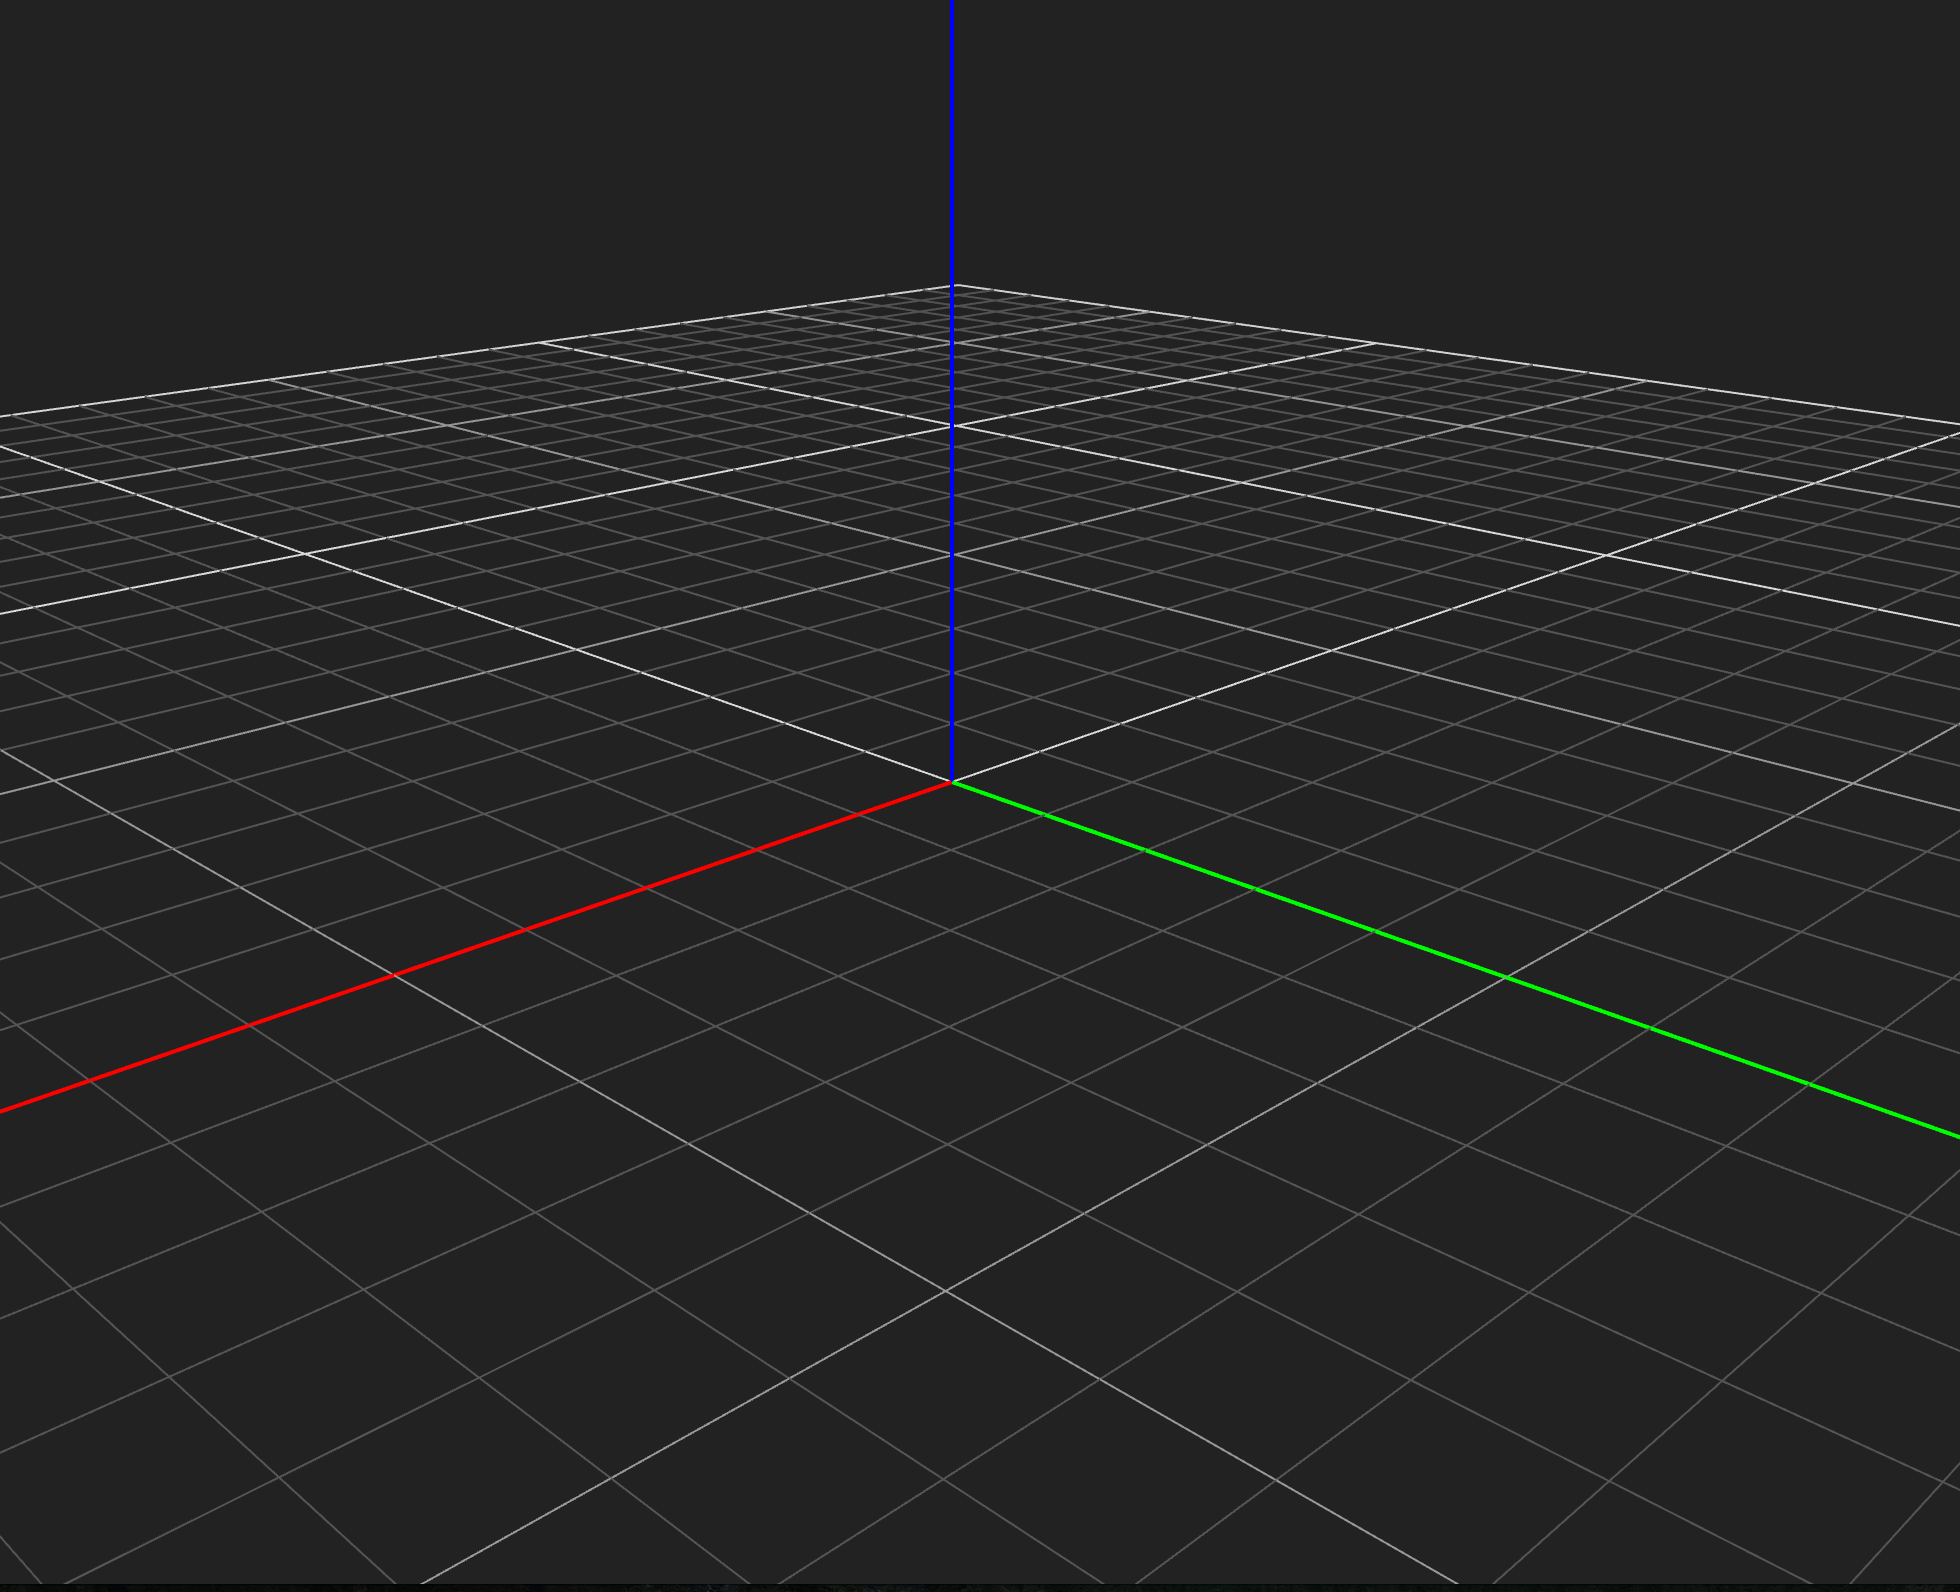
\includegraphics[width=1\columnwidth]{03-architecture_overview_coordinate_system}
  \caption{An empty scene showing the coordinate system.}
  \label{fig:architecture_overview_coordinate_system}
\end{figure}

\subsubsection{Platener Pipeline}

The Platener Pipeline plugin is the main computation unit. The plugin defines
multiple {\fabmethod}s. A {\fabmethod} is a conversion approach of a
\threedmodel. Multiple components, which can manipulate the input model, are
chained after another to produce 2D- or 3D-output. For example construction
plans for the original input model as {\svgfile}s.

\subsubsection{Node Visualizer}

We visualize the results of the Platener Pipeline plugin in the WebGL view. The
Node Visualizer plugin renders the results of each component of each
{\fabmethod} respectively.

\myNotes{add figure of a visualized model in wireframe mode (something fancy)}

\subsubsection{Scoring}

When multiple {\fabmethod}s are run, we want to choose the best fitted
conversion as output. Thus each {\fabmethod} is scored by a method-specific
scoring algorithm. This plugin provides these scoring algorithms.

\subsubsection{Solution Selection}

This plugin utilizes the Platener Pipeline plugin and the Scoring plugin to run
and evaluate all {\fabmethod}s. It outputs the result of the {\fabmethod} with
the best score and notifies the Dispatcher.

\subsubsection{Isolated Testing}

While we worked at different stages of a linearly executed {\fabmethod} in
parallel, we needed a mechanism to test each component of the {\fabmethod}
before its preceeding or succeeding components were finished. The Isolated
Testing plugin provides an isolated environment, which allows to execute a
single component of a {\fabmethod} with pre-defined input.

% - working in parallel, while needing inputs of work in progress - validate &
% visualize test scenarios for separate pipeline steps (components of a
% \fabmethod) - provide input for a given step and compute/ render results for
% just that step


\subsection{Platener Pipeline}

\begin{enumerate}
\item Overview/ Purpose/ Plugin Structure

\item conversion strategies and logic

  \begin{itemize}
  \item logic only (ui -> other plugin, frontend)
  \item processing broken into steps
  \item composable into fabrication methods = execute steps in sequence, use
    results from previous step, to go on = conversion strategy

  \item typical pipelining problem \myNotes{look up typical pipelining problems}
  \item in general we have to: clean mesh, indexing, find structure (understand
    the model), convert structures (plates and joints), export
  \item different methods may to these things differently (stacked plates vs.
    inherent plates)

  \end{itemize}

\item Pipeline Steps

  \textbf{What are pipeline steps?}

  \begin{itemize}
  \item processing unit on model data (or abstraction of it)
  \item indepentend from each other, a single task
  \item break down problem into sequential sub problems (working with
    abstractions, generating assumptions -> understand problems better, work in parallel)
  \item improve debugging experience (trace errors in decouple computation
    units, also its hard to see how vertices are from
    looking at the memory, --> see next bullet)
  \item store state of each step separately, to later render a debugging view of
    the state (like timetravel for manipulations on the model)
  \item but keep rendering apart from logic -> NodeVisualizer
  \item isolated computing -> isolated testing (nice!)
  \end{itemize}

  \textbf{How are they used in Platener Pipeline?}

  \begin{itemize}
  \item pipe steps -> build up a pipeline from composition
  \item final result will be exported from the browser
  \item a pipeline makes up a conversion strategy
  \item conversion strategy share certain subproblems -> reusable code
  \item \myNotes{as steps solve the real algorithmic problems, we dedicated separate
    chapters to them. look at chapters ??}
  \end{itemize}

  \textbf{Where to be found in the code?}

  \begin{itemize}
  \item Plugins Package
  \item organized in subdirs (remember, separate npm package)
  \item step factories -> configure steps for different strategies, inject
    dependencies and state, lazy loading
  \end{itemize}

\item Fabrication Methods
  \begin{enumerate}
  \item Plate Method
    \begin{itemize}
    \item hull and surface constructions
    \item find plates in the model (inherent), build plates from surfaces
      (extruding)
    \item intersect plates (graphing)
    \item and join connected plates (finger joints)
    \item \myNotes{figure here}
    \item \myNotes{listing showing how to concat/ pipe steps}
    \item main parts of algorithm explain in chapters lukas, klara, dimitri, deus
    \end{itemize}

  \item Stacked Plates Method
    \begin{itemize}
    \item volume approximation
    \item stack flat plates to rebuild the object
    \item preserve form, look and feel, details
    \item loose functional aspects
    \item connect via shafts (click together) or use glue
    \item \myNotes{figure here}
    \item main parts of the algorithm explained in chapters lukas
    \end{itemize}

  \item Classifier Method
    \begin{itemize}
    \item advanced technique, combining intense mesh analysis and construction
      techniques of known geometries
    \item pros: convert noisy models, local conversions: because different local
      geometries may be better converted with different techniques, e.g. stacked
      vs. fingerjoints. we can evaluate better (scoring locally also!). global
      conversions and evaluations are error prone. classifier method could
      provide a rather robust conversion strategy. \myNotes{WHY CLASSIFIERS?}
    \item work in progress
    \item we can currently use primitive detection algorithms
    \item \myNotes{figure of detected cylinder in model}
    \item main parts of the algorithm at the end of paper (classification
      chapter, ransac stuff)
    \end{itemize}
  \end{enumerate}

\item Immutable Pipeline State

  \begin{enumerate}
  \item Overview/ Purpose
    \begin{itemize}
    \item no unwanted mutations (nice persisting of intermediate results from
      pipelinesteps)
    \item later steps work on data form previous steps
    \item code was not written immutable throughout the project -> changing data
      will result in wrong visualizations of previous steps by the node
      visualizer, because rendering performs AFTER all computations are done
    \end{itemize}

  \item Immutability
    \begin{itemize}
    \item \myNotes{explain principle. have more pros and cons.}
    \item structural data sharing -> unfortunately, not for us yet, but thats
      the concept :)
    \item http://jlongster.com/Using-Immutable-Data-Structures-in-JavaScript
    \item http://stackoverflow.com/questions/10034537/persistent-vs-immutable-data-structure
    \item enforces certain code style, mutability may be easier to write
    \item slow downs maybe (performance)
    \end{itemize}

  \item Implementation Details
    \begin{itemize}
    \item PipelineState class
    \item mutable and immutable state properties
    \item providing a clone method for stored properties, because code throughout the project shall
      not necessarily be written immutable (hard to obey, --> cg dev orientated,
      c++ is not immutable)
    \item immutable properties implement the clonable protocol
    \item provide immutable in one spot -> state creation
    \item define a schema (all props always available, having defaults) ->
      reduce faults when accessing data
    \item add listing which defines the schema for stacked plates
    \item accessing undefined values will give us a warning (again, like
      protocols enforcing interface structure, reducing faulty data access)
    \item somehow a persistence api (see stackoverflow link)
    \end{itemize}
  \end{enumerate}

\item Pipeline Implementation

  \begin{enumerate}
  \item the pipeline works as follows...
    \begin{itemize}
    \item Pipeline class
    \item pipe interface for Step factories (compare listing above, stacked method)
    \item create state factory -> use composition to persist intermediate results
      (state is later accessed by node visualizer)
    \item reduce approach -> pipe last state into next step to produce new state
    \item show a listing of pseudo code, explaining how the pipeline works
    \item benchmarking (measure time for intermediate steps vs whole processing)
    \end{itemize}

  \item it can be reused (because pipelining is a generic concept)
    \begin{itemize}
    \item classifier graph (classification method)
    \item isolated testing (injectable pipeline)
    \end{itemize}
  \end{enumerate}

\end{enumerate}

\subsection{Solution Selection}

\begin{enumerate}
\item WHAT?
  \begin{itemize}
  \item Selecting the best estimated solution by default.
  \item execute all classification methods
  \item use scorer plugin to evaluate each conversion after computation
    (globally evaluated, local converted geometries could be really bad)
  \item provide list of solutions associated with a score
  \item solution with max score is provided as default download
  \end{itemize}

\item WHY?
  \begin{itemize}
  \item strategies not mergeable in current state (would be future work to bring
    them together, like classifier method approach)
  \item so we want to select the method as default, which may has done the job
    most correctly (scoring)
  \item also scoring helps to get an idea of the quality of conversion without
    looking at the result (visually) -> used in headless mode, batch processing
    we could detect poorly converted objects to have a detailed look of what
    went wrong (getting development forward, yay!)
  \end{itemize}

\item MEASUREMENTS and HOW SCORING?
  \begin{itemize}
  \item \myNotes{look at screenshots and describe in short what we thought,
      would be nice measurements}
  \item scoring plugin: per measurement per classification method -> score
    method
  \item then adding all measuremnt scores per classification together
  \item assign score to the solution
  \end{itemize}

\item HOW SOLUTION SELECTION?
  \begin{itemize}
  \item combining plugins platener pipeline and scorer
  \item promised -> loop overall pipelines of classification methods
  \item promised -> then apply scoring
  \item when failure, catch and report nicely in evaluationDidFail hook (so
    fronend can notify users, no hard failure)
  \item results pushed back to system via evaluationDidFinish hook
  \end{itemize}
\end{enumerate}

\subsection{Node Visualizer}

\begin{enumerate}
\item Overview
  \begin{itemize}
  \item meshlib library for model representation
  \item convert meshlib face vertex mesh to three js notation
  \item render imported model and its manipulated forms with threejs
  \item use data from platener pipeline plugin
  \item the dispatcher implements solutionselectiondelegate protocol, which
    lets the node visualizer render the data after it was computed (see listing
    ??, above)
  \end{itemize}

\item Visual Debugging
  \begin{itemize}
  \item Rendering into WebGL only in NodeVisualizer
  \item other plugins could also do it
  \item but keep visualization of processed model in one place
  \item for each pipeline step, access its state data in a separate
    visualization
  \item step through, like explained in walkthrough chapter
  \end{itemize}

\item Visualizer and Visualizations
  \begin{itemize}
  \item Visualization class, constructs a drawable (THREE.object3d)
  \item injects drawable into root node of NodeVisualizer plugin
  \item Renderer will render it
  \item Visualizer class, wrapper managing visibilities of visualizations
  \item toggable through frontend
  \item visualizersets -> group visualization for a fab method (not all
    fabmethods have all steps, thus dont need all visualizations)
  \end{itemize}

\item Interwoven with Platener Pipeline
  \begin{enumerate}
  \item Role of Immutability
    \begin{itemize}
    \item \myNotes{(show example of how shapes have fingerjoints)}
    \item shapes (find outlines of possible plate geometries)
    \item fingerjoints are added to shapes in a later step
    \item shapes visualization also shows fingerjoints now (no timetravel - bad
      debugging (we cannot see if shapes did something wrong))
    \item data will not be changed if immutable (yes!!)
    \end{itemize}

  \item Extracting Intermediate Data of the Pipeline
    \begin{itemize}
    \item we access solutions (state per fabmethod)
    \item PipelineVisualization parent class
    \item convert state to plain object for fast access
    \item \myNotes{listing for PipeVis}
    \item each visualization extending pipeline viz only has to implement a
      single method, returning a drawable threejs object
    \end{itemize}
  \end{enumerate}
\end{enumerate}

\subsection{Isolated Testing}

\begin{enumerate}
\item WHY?
  \begin{itemize}
  \item validation of data/ conversion
  \item parallel working (make mock data with certain assumptions)
  \item isolated testing in real environment (test env is not representative,
    integration tests with manual evaluation (look at the visual results))
  \end{itemize}

\item Static Input
  \begin{itemize}
  \item build data like assumed for the step we test
  \item not that easy: many cross references, after certain steps, complex
    data...
  \item hard to build by hand, we had to use previous steps and serialize the
    step data
  \end{itemize}

\item Testables
  \begin{itemize}
  \item 1 step, 1 static input, certain test purpose
  \item a single integration test
  \item e.g. classify a single shape as plane in classify geometry step
  \end{itemize}

\item Implementation
  \begin{itemize}
  \item reusing concept of pipeline
  \item small changes: allow only a single step, get input from testable
  \end{itemize}

\item Conclusion
  \begin{itemize}
  \item not perfected/ technically mature
  \item mostly we evaluated by dropping in models
  \item but wrongly executed previous steps may have corrupted our assumptions
  \item thats why working out nice testables would be worth it!
  \end{itemize}
\end{enumerate}

\section{Client Package}
% ************************************************

\subsection{Overview - Custom Frontend Code}

\begin{itemize}
\item when convertify framework, client is freespace to evolve yaself
\item look and feel of the application
\item task: connect logic to ui (speak with dispatcher) and build ui
\item free choice of frontend framework (we take redux + react), but nothing
  against jquery or angular or backbone or ...
\item e.g. laser origami or brickify would choose a completely different
  implementation of client -> custom per application
\item react by facebook, redux by dan abramov, like flux architecure -> uni
  directional dataflow, explicit state changes, data driven -> reduce side
  effects and be efficient in coding and trace down errors easily
\item \myNotes{diagram which shows benefits of flux architecture vs no flux
    arch, look at intro vids for redux from dan abramov}
\end{itemize}

\subsection{React Templates}

\begin{itemize}
\item show html tree graph and how data communication goes wild when talking
  with siblings
\item ideally dumb components (dont know where data is coming from, just display
  it)
\item stateless, components directory
\item WIP: before no redux, so there are some mixed up components left :S
\item show short example how a dump component looks like, \myNotes{listing!}
\end{itemize}

\subsection{Redux Data-driven Control Flow}

\begin{enumerate}
\item Redux `dispatch` and state
  \begin{itemize}
  \item one state container
  \item functional, no side effects
  \item maybe copy or reference redux description (just explain why its awesome)
  \item injected into react via context
  \end{itemize}

\item Smart Containers
  \begin{itemize}
  \item connect to state
  \item containers know where data is from (vs dump components)
  \item fitler and preprocess raw data, setup interaction events to trigger
    actions
  \item give data and callbacks to a component (they setup the actual ui, but
    contain no visible elements themselves)
  \item \myNotes{listing show how to connect and use component from other
      listing}
  \end{itemize}

\item Manage Async Plugin Hell
  \begin{itemize}
  \item as described before, plugin data is not available on load
  \item we can use Dispatcher and redux dispatch combined
  \item protocols -> state change in plugins -> dispatch -> state change in
    frontend
  \item no polling or observing of data, fully reactive (system -> client communication)
  \item as client has access to bundle, we can call interfaces exposed by
    protocols (client -> system communication)
  \end{itemize}
\end{enumerate}

\section{Server Package}
% ************************************************

\subsection{Overview - Custom Server Code}

\begin{itemize}
\item like client, can have custom implementations
\item we have caching and cli (headless version of application)
\item requires isomorphic code: execute on client and server equally
\item \myNotes{isomorphic means...}
\item threejs, polyfills, \myNotes{...}
\end{itemize}

\subsection{Model Cache}

\begin{itemize}
\item idea: build up repository of models when users interact with it
\item taken from brickify: uploading meshlib version of model
\end{itemize}

\subsection{Test Pipeline}

\begin{enumerate}
\item WHY do we have a Test Pipeline?
  \begin{itemize}
  \item robustness tests
  \item batch processing
  \item headless version for integration with other projects
  \item failure detection because of diversity of objects
  \end{itemize}

\item Headless Conversion of Objects
  \begin{itemize}
  \item run solutionselection plugin also
  \item but dispatcher is setup a bit differently
  \item no recomputation, no grid, no visualizer
  \item scene manager will not render anything (unless, WIP we exchange webgl
    rendering with headlessgl to produce screenshots of each conversion)
  \item cli tool -> safe results into directories
  \end{itemize}

\item Reports
  \begin{itemize}
  \item = extended console logs
  \item show how conversion was going
  \item display failures, status, progress
  \item in the end: sum up + give stats
  \item WIP: current problems: not all conversions are garbage collected
    correctly, will run out of memory after some conversions -.- (maybe nobody
    has to know about that)
  \end{itemize}

\item Benchmarks
  \begin{itemize}
  \item xxx testmodels
  \item we proposed mostly stacked as the best solution
  \item too many arbitrary forms hindered plate conversion
  \item just shows conversion stats (maybe all models vs box category only)
  \item \myNotes{measure times for conversions and evaluate}
  \end{itemize}
\end{enumerate}


\fi

\end{document}

%%% Local Variables:
%%% mode: latex
%%% TeX-master: "../ClassicThesis"
%%% TeX-command-extra-options: "-shell-escape"
%%% End:
